\chapter{Related Work}

\section{Pose Estimation}
% first: single images only, no video

While there are many different approaches for pose estimation, one of the most widely used in the literature until recently was the \textit{Pictoral Structure Framework}.
In the following section, the foundation of this framework will be explained, along with some additions to it.
Afterwards, deep learning based methods became dominant in the field of pose estimation which is why they will be explained in the subsequent section.

\subsection{Pictoral Structure Framework}
In 1973, \cite{fischler_representation_1973} presented a general framework for object recognition problems, including pose estimation.
The so called \textit{Pictoral Structure Framework} is comprised of parts, connected by \textit{spring-like connections}.
In the context of pose estimation, they used the term \textit{part} to be synonymous with \textit{limb}.
A part is defined by a collection of parameters $l_i$ which could include center coordinates and rotation.
The connection between two parts is modelled using a mechanism inspired by physical springs.
Similar to a string, such a connection can be relaxed or be under tension.
This expresses how realistic a certain connection is, based on the amount of tension required to connect two parts.

The graph that is created that way then models the desired object, for example the pose or facial features of a human, and is also referred to as a \textit{deformable structure}.
In the context of pose estimation, limbs are modelled as parts, connected together at the joints.

The output of the alorithm is expressed as $L = (l_0, l_1, \dots, l_n)$, called the \textit{configuration} of all parts $l_i$.
To compute the optimal configuration, the authors proposed the following minimization problem:

\begin{equation}
    \label{eq:energy-minimization}
    L^* = \argmin_L \left(\sum_{i=0}^n m_i(l_i) + \sum_{(v_i, v_j) \in E} d_{ij}(l_i, l_j)\right).
\end{equation}

$m_i$ is a function evaluating the placement of part $i$ at configuration $l_i$.
This is also often referred to as the \textit{unary} term.
$d_{ij}$ measures the mismatch when parts $i$ and $j$, which are connected, are placed according to $l_i$ and $l_j$ respectively.

Minimizing the energy function is computationally expensive since the space of possible positions for each part spans the entire image.
% ------ GENERAL OBJECT RECOGNITION FRAMEWORK ----------
According to \cite{felzenszwalb_pictorial_2005}, there are methods using heuristics to make the computation more efficient but they do not find optimal solutions.
They proposed to transform the problem into a statstical framework and solve it by estimating a posterior distribution.

One advantage of this statistical model is that the parameters can then be estimated using training examples, similar to the principles of learning presented in \sref{sec:neural_networks}.
Also, it is trivial to get multiple solutions to the minimization problem by sampling the posterior distribution as opposed to a single solution with the energy minimization approach.

The authors model the problem as follows.
Let $p(L \mid I, \theta)$ be the desired posterior distribution, where $\theta$ is a set of model parameters and $I$ is the image.
When applying Bayes' formula, one can express the posterior as:

\begin{equation}
    p(L \mid I, \theta) \propto p(I \mid L, \theta) p(L \mid \theta).
\end{equation}

The likelihood $p(I \mid L, \theta)$ is approximated as $\prod_{i=1}^n p(I \mid l_i, \theta_i)$.
This approximation, however, is bad if recognized parts overlap, which is often the case when detecting human limbs.
This problem is often referred to as \textit{double counting} and is one of the most prominent error of Pictoral Structure based models.
The authors tackle this problem by sampling multiple times from the posterior and evaluating them using a separate measurement.

To approximate the prior distribution $p(L \mid \theta)$ the authors utilize the joint distribution of a tree structured Markov random field.
This tree is also referred to as the \textit{kinematic pose prior} since it encodes prior information of how limbs should be connected together.
The vertices are modeled by $l_i$ and the edges show connections between the different parts. 
They set the denominator to $1$ because they argue that it can be constant if only relative position between parts are of importance:

\begin{equation}
    \begin{split}
        p(L \mid \theta) 
        &\propto \frac{\prod_{(i,j) \in E} p(l_i, l_j \mid \theta)}{\prod_{i \in V} p(l_i \mid \theta)^{\text{deg} ~ v_i -1}} \\
        &\propto \prod_{(i, j) \in E} p(l_i, l_j \mid \theta).
    \end{split}
\end{equation}

This then leads to the following approximation of the posterior distribution:

\begin{equation}
    \label{eq:pictoral-posterior-general}
    \begin{split}
        p(L \mid I, \theta) 
        &\propto p(I \mid L, \theta) p(L \mid \theta) \\
        &\propto \prod_{i=1}^n p(I \mid l_i, \theta_i) \prod_{(i, j) \in E} p(l_i, l_j \mid \theta).
    \end{split} 
\end{equation}

To show the equivalence to the original energy minimization problem, the authors take the formula presented in \eref{eq:pictoral-posterior-general} and apply the logarithmic function. Then, they negate the result.
This then leads to the following formulation:

\begin{equation}
    \label{eq:neg-log-posterior}
    \begin{split}
        &-log \left( \prod_{i=1}^n p(I \mid l_i, \theta_i) \prod_{(i, j) \in E} p(l_i, l_j \mid \theta) \right) \\
        &= -log \left( \prod_{i=1}^n p(I \mid l_i, \theta_i) \right) - log \left( \prod_{(i, j) \in E} p(l_i, l_j \mid \theta)\right) \\
        &= \sum_{i=1}^n -log ~ p(I \mid l_i, \theta_i) + \sum_{(i, j) \in E} - log ~ p(l_i, l_j \mid \theta).
    \end{split}
\end{equation}

When comparing \eref{eq:neg-log-posterior} to \eref{eq:energy-minimization} it is easy to see that $m_i(l_i) = - log ~ p(I \mid l_i, \theta_i)$ and $d_{ij}(l_i, l_j) = p(l_i, l_j \mid \theta)$.

After presenting the statistical framework for general object recognition tasks, the authors explain their approach to pose estimation using this framework.
First, they specify that the input image needs to be a binary image where the person is separated from the background.
Then, the objective is to maximize the number of foreground pixels covered by the detected parts in their calculated configuration.
A visualization of this process can be seen in \fref{fig:felzenszwalb-overview}.

\begin{figure}[htb!]
    \centering
    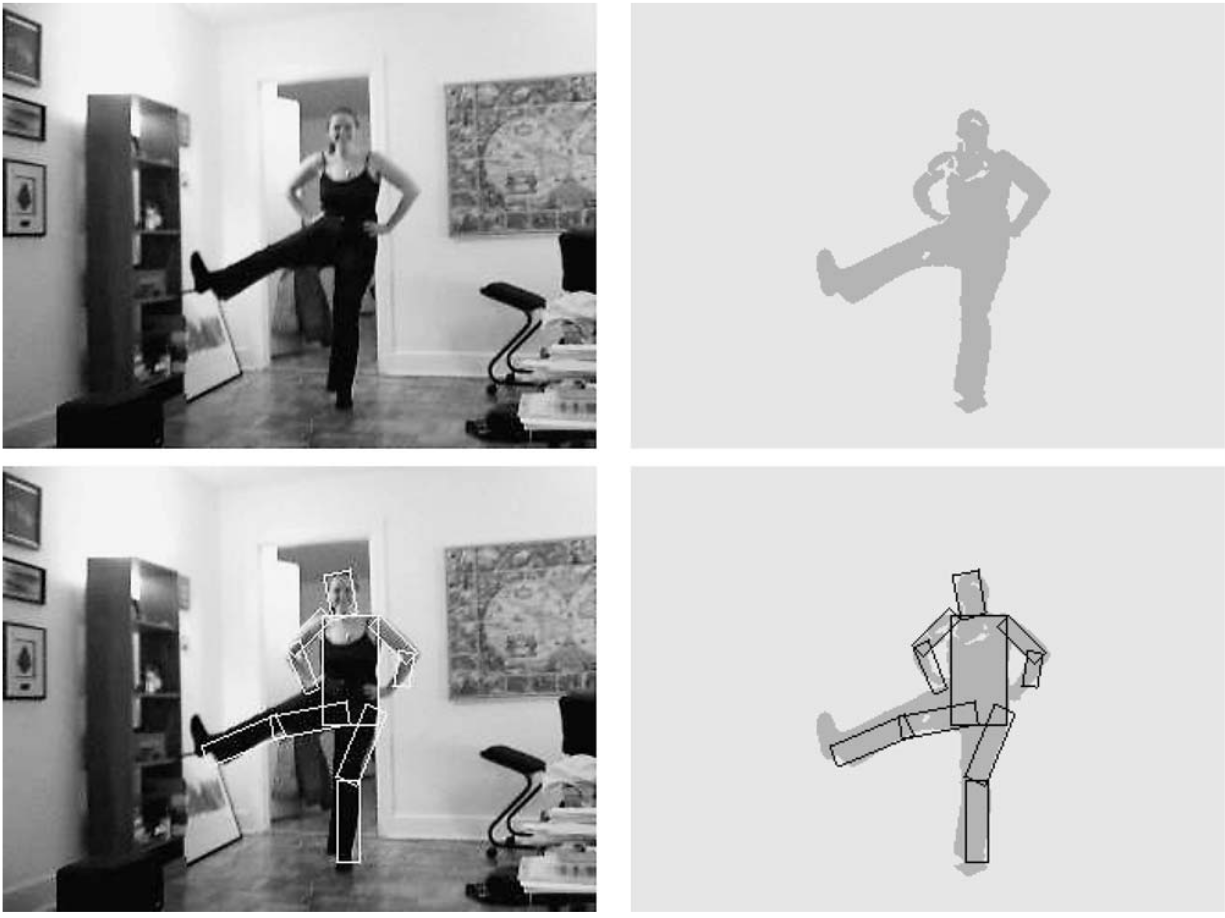
\includegraphics[width=0.8\textwidth]{felzenszwalb-overview.png}
    \caption{Overview of pose matching algorithm. \textbf{Upper left}: Original image. \textbf{Upper right}: binary image where foreground pixels (containing the human figure) are separated from the background. \textbf{Lower right}: One result from matching the limb rectangles to maximize the amount of foreground pixels covered. \textbf{Lower left}: Final result with estimated pose layered on top of original image. Image taken from \cite{felzenszwalb_pictorial_2005}.}
    \label{fig:felzenszwalb-overview}
\end{figure}

The authors model the human pose as a collection of $10$ different parts. 
Two parts per arm and leg as well as one torso and one head part \fref{fig:felzenszwalb-overview}.
Each part configuration $l_i = (x_i, y_i, s_i , \varphi_i)$ contains the $x$ and $y$ coordinate of the center of the rectangle representing the part.
In addition, $s_i \in [0,1]$ defines the length of the rectangle and $\varphi_i$ its rotation.
The width is fixed.

To model $p(I \mid l_i, \theta_i)$ they use the formula in \eref{eq:felz-unary} which utilizes $\theta_i = (q_1, q_2)$.
$q_1$ is the probability of pixel inside $l_i$ being a foreground pixel whereas $q_2$ is the probability of pixels closely around $l_i$ being foreground pixels.
The area around $l_1$ is referred to as $area_2$ whereas the area of $l_i$ is referred to as $area_1$.
$count_i$ referres to the number of foreground pixels in $area_i$ and $t$ is the total number of pixels in the image.

\begin{equation}
    \label{eq:felz-unary}
    \begin{split}
        p(I \mid l_i, (q_1, q_2)) = &q_1^{count_1} * (1 - q_1)^{(area_1 - count_1)} \\ 
        &* q_2^{count_2} * (1 - q_2)^{(area_2 - count_2)} \\ 
        &* 0.5^{(t - area_1 - area_2)}
    \end{split}
\end{equation}

Also, they smooth the distribution to prevent peaks by using the principle of annealing with a constant factor $T$ \eref{eq:smoothed}.
This is important because a distribution with strong peaks is more likely to return similar results when sampled from.
As discussed earlier, sampling is needed because of the approximation of the unary term the authors used and its problem with overlapping limbs.
A distribution with too strong peaks would not allow for sufficiently different pose samples.

$\theta_i$ is then estimated using mean values from annotated training data points while $T$ is set to $10$.

\begin{equation}
    \label{eq:smoothed}
    p(I \mid l_i, \theta_i) \propto p(I \mid l_i, \theta_i)^{\frac{1}{T}}
\end{equation}

\begin{figure}[htb!]
    \centering
    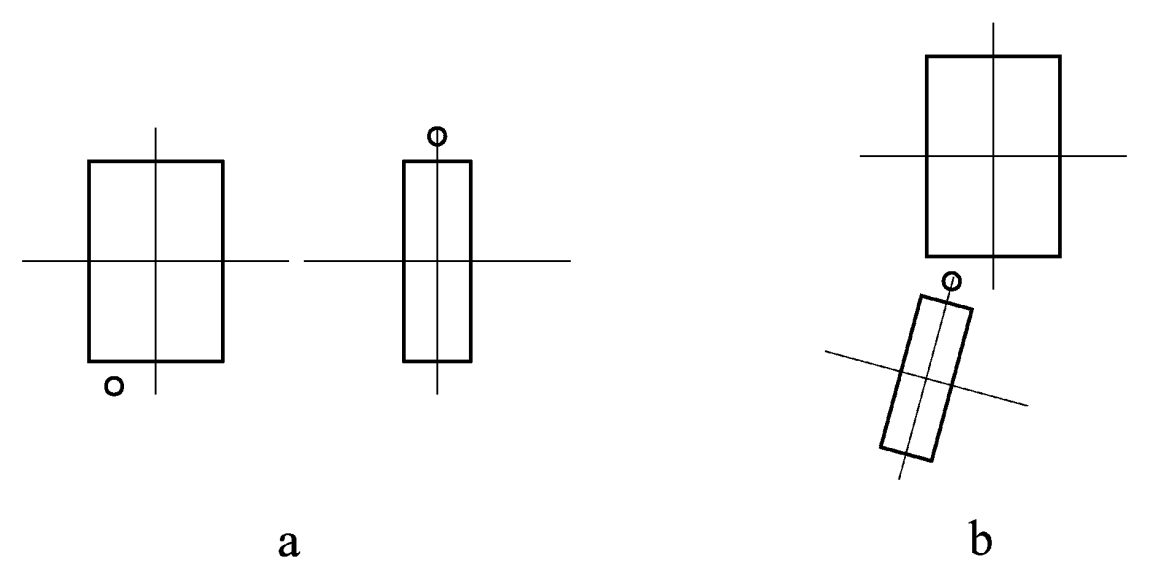
\includegraphics[width=0.8\textwidth]{limb-connection.png}
    \caption{Visualization of connecting limbs. \textbf{a}: Two limbs in their own coordinate system. The circles indicate connection joints. \textbf{b}: Possible, anatomically plausible connection. Image taken from \cite{felzenszwalb_pictorial_2005}.}
    \label{fig:limb-connection}
\end{figure}

Next, the authors model the prior $p(L \mid \theta)$.
Each spatial relation $p(l_i, l_j \mid \theta)$ between two parts is modelled in the following way:
First, each part is placed inside its own coordinate system with the origin being the center point of the part (see \fref{fig:limb-connection}a).
The connection point (joint) between parts $i$ and $j$ is defined as $(x_{ij}, y_{ij})$ in the coordinate system of part $i$ and as $(x_{ji}, y_{ji})$ in the coordinate system of part $j$.
When transformed to the image coordinate system, these points should be as close together as possible (see \fref{fig:limb-connection}b).
The authors express this using Gaussian distributions:

\begin{equation}
    \begin{split}
        N((\hat{x}_i - \hat{x}_j), 0, \sigma^2_x) \\
        N((\hat{y}_i - \hat{y}_j), 0, \sigma^2_y),       
    \end{split}
\end{equation}

where $\hat{x}_i$ and $\hat{y}_i$ are transformations of the joint position into the image coordinate system:

\begin{equation}
    \begin{bmatrix}
        \hat{x}_i \\ 
        \hat{y}_i
    \end{bmatrix}
    =
    \begin{bmatrix}
        x_i \\ 
        y_i
    \end{bmatrix}
    + s_i R_{\varphi_i}
    \begin{bmatrix}
        x_{ij} \\ 
        y_{ij}
    \end{bmatrix}.
\end{equation}

$\hat{x}_j$ and $\hat{y}_j$ are computed analogously.
$R_{\varphi_i}$ is a matrix which rotates around the origin for $\varphi_i$ radiants.
Additionaly, the authors define that the difference between $s_i$ and $s_j$ should be close to zero as well.
Again, this is modelled using a Gaussian distribution:

\begin{equation}
    N((s_i - s_j), 0, \sigma^2_s).
\end{equation}

Lastly, the authors specify that the difference between the two relative angles $\varphi_i$ and $\varphi_j$ be close to a parameter $\varphi_{ij}$.
They use a von Mises distribution, given by

\begin{equation}
    M(\theta, \mu, k) \propto \exp (k \cdot \cos (\theta - \mu)).
\end{equation}

A von Mises distribution can be thought of as a normal distribution around a circle, which is why the authors use it for periodic input like gradients.
Using $\mu = \varphi_{ij}$ they specify the constrained described earlier.
The parameter $k$ determines how strong the peak at $\varphi_{ij}$ should be or, in other words, how constrained the joints should be.

In summary, each spatial relation is expressed in the following way:

\begin{equation}
    \begin{split}
        p(l_i, l_j \mid \theta) 
        &= p(l_i, l_j \mid c_{ij}) \\
        &= N((\hat{x}_i - \hat{x}_j), 0, \sigma_x^2) \\
        &* N((\hat{y}_i - \hat{y}_j), 0, \sigma_y^2) \\
        &* N((s_i - s_j), 0, \sigma_s^2) \\
        &* M((\varphi_i - \varphi_j), \varphi_{ij}, k).
    \end{split}    
\end{equation}

The prior parameters $c_{ij}$ are then given by $c_{ij} = (x_{ij}, x_{ji}, y_{ij}, y_{ji}, \sigma_x, \sigma_y, \sigma_s, \varphi_{ij}, k)$ and are estimated using maximum likelihood estimation.

% ----- Short evaluation
The authors merely provide example images instead of a quantitative analysis.
This is most likely because of the lack of benchmark datasets available at the time.
They labeled $10$ images by hand and used these to estimate the parameters.
Then, for each of their unlabeld test images, they sampled $200$ poses and calculated the Chamfer distance, which measures the binary correlation.
The best pose with regards to the Chamfer distance is then returned.
Some example images can be seen in \fref{fig:pictoral-examples}

\begin{figure}[htb!]
    \centering
    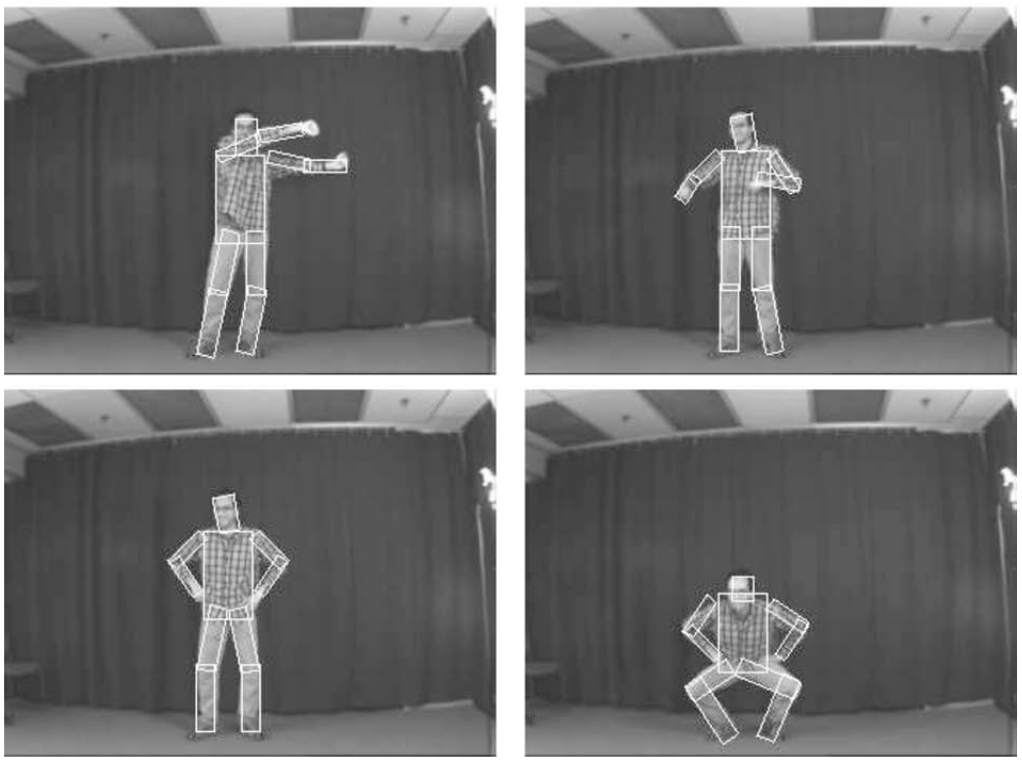
\includegraphics[width=0.8\textwidth]{pictoral-examples.png}
    \caption{Example of poses estimated by the statistical framework. Image taken from \cite{felzenszwalb_pictorial_2005}.}
    \label{fig:pictoral-examples}
\end{figure}

\subsubsection{Approaches for parts detection}
\label{sec:pose-andriluka}
Over the years, many approaches build on top of \cite{felzenszwalb_pictorial_2005} by improvig parts of the framework.
One approach, where the parts detector was improved upon, is presented in the following section.

In \cite{andriluka_pictorial_2009}, the authors propose a different appearance model $p(I \mid L, \theta)$, which is based on individual parts detectors.
\cite{felzenszwalb_pictorial_2005} used background separation to extract the silhouette of the subject from the background.
Then, the objective was to configure the parts in such way that the covered foreground area was maximized (see \eref{eq:felz-unary}).
This resulted in a large search space since all different rotations and scalings for each part need to be placed inside the foreground area in order to evaluate the overall fit.
The authors in \cite{andriluka_pictorial_2009} limit the search space by using a detected \textit{parts evidence map} $d_i$ for each part $i$.
An example evidence map can be seen in \fref{fig:parts-evidence}.
These evidence maps are the result of individual parts detectors trained on annotated images such as presented in \fref{fig:parts-annot}.

\begin{figure}
    \centering
    \subfloat[Parts-annotated example image.\label{fig:parts-annot}]{%
        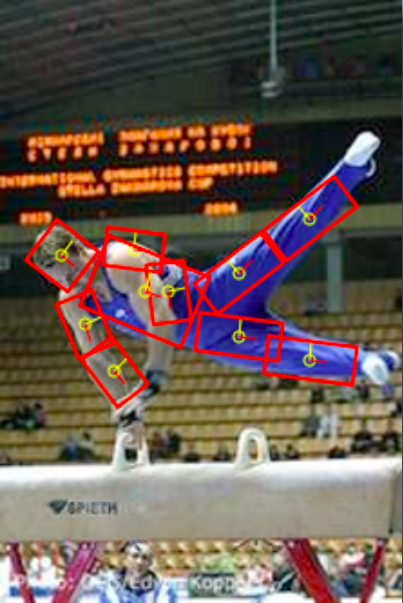
\includegraphics[height=150px]{poseparts.png}
    }
    \hspace{20px}
    \subfloat[Part evidence map for part \textit{head}. Notice the peak (in red) where the head is in the left image.\label{fig:parts-evidence}]{%
    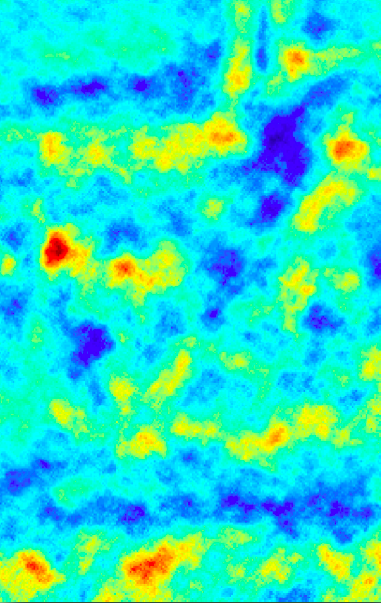
\includegraphics[height=150px]{partevidence.png}
}
    \caption{Images taken from corresponding talk to \cite{andriluka_pictorial_2009}.}
\end{figure}

% Descriptors
The authors compute dense \textit{shape context descriptors} \cite{belongie_shape_2002} for each training image.
This local descriptor takes gradients of edge pixels into account and discretizes them into bins in a log-polar histogram.
The authors chose $12$ bins for the location where the gradients are put inside $8$ bins, resulting in a $96$ dimensional descriptor for each sampled point.
Descriptors with a center point inside a part bounding box given by the annotation are then concatenated and used as positive training examples to train the parts detectors.

% Detectors
For detectors, the authors use the concept of \textit{boosting} where the decisions of many weak classifiers are combined into a strong classifier \cite{freund_short_1999}.
Specifically, the authors use the \textit{AdaBoost} algorithm proposed by \cite{freund_decision-theoretic_1997}.
Each weak detector takes a bin from the feature vector and compares it to a threshold.
The sign of the result is then used as the output of the weak detector following

\begin{equation}
    h_t(\bm{x}) = sign(\xi_t (\bm{x}_{n(t)} - \varphi_t )),
\end{equation}

where $\bm{x}$ is the feature vector, $\xi_t \in \{-1, 1\}$ and $n(t)$ is the index of the bin, which is used to compare to $\varphi_t$.
The authors do not, however, specify how to set $\xi_t$ or which threshold $\varphi_t$ was used.

Combining $t$ weak detectors by summing over the weighted outputs, the complete part detector for part $i$ is given by 

\begin{equation}
    H_i(\bm{x}) = sign\left(\sum_t a_{i,t} h_t(\bm{x})\right)
\end{equation}

According to the authors, $a_{i,t}$ are weights learned by each weak detector.
To fit the parts detectors into the Pictoral Structure Framework, the authors compute a pseudo-probability based on the part detectors:

\begin{equation}
    p(d_i \mid l_i) = max \left(\frac{\sum_t a_{i,t} h_t(\bm{x}(l_i))}{\sum_t a_{i,j}}, \epsilon_0 \right).
\end{equation}

$\bm{x}(l_i)$ is the feature vector for part $l_i$ whereas $\epsilon_0$ is set to $10^{-4}$.
The authors claim that this pseudo-probability achieves good results in practice.

% Appearance model Pictoral Structure Framework
Lastly, the authors make two assumptions in order to embed the parts detectors into the Pictoral Structute Framework.
First, different part evidence maps $d_i$ are independent from each other given $L$.
Second, $d_i$ only depends on $l_i$ on not on other parts configurations.
This leads to the following likelihood

\begin{equation}
    p(I \mid L, \theta) = p(D \mid L) = \prod_{i=0}^N p(d_i \mid l_i),
\end{equation}

where $N$ is the number of parts to detect in the given image.

% Evaluation
\label{sec:andriluka-eval}
The authors use two datasets to evaluate their model.
The \textit{Buffy} dataset provides annotated upper-body poses from $3$ episodes of the TV series \textit{Buffy The Vampire Slayer} \cite{ferrari_progressive_2008}.
Also, for evaluating full-body poses, they used the \textit{Iterative Image Parsing} dataset provided by \cite{ramanan_learning_2007}

As an evaluation metrc, the authors use \textit{Percentage of Correct Parts (PCP)}, proposed by \cite{ferrari_progressive_2008}.
For each annotated body part, PCP is calculated by first computing the length of the ground truth body part $l_{gt}$.
Then, a threshold value $t_{gt} = 0.5 \cdot l_{gt}$ is defined as half the length of the segment.
If both endpoints of a prediction fall within $t_{gt}$ radius of their ground truth annotation the part is considered detected.

First, they compare their upper-body model to \cite{ferrari_progressive_2008}.
In contrast to \cite{ferrari_progressive_2008}, however, the authors also compute PCP for each part, whereas \cite{ferrari_progressive_2008} only provide the overall accuracy of $57.9\%$.
Using the pose dataset of \cite{ramanan_learning_2007} for training the pose priors and part detectors, the authors achieve an overall accuracy of $71.3\%$.
They notice that, while torso, head and upper arm accuracy is fairly high (from $78\%$ for upper arm to $95.9\%$ for head), forearm accuracy ($40\%$) was significantly lower.
They argue that is is due to the challenging nature of the dataset.
Also, forearm parts are smaller, making it more difficult for parts to be considered correct.
The authors also tried exclusively using frames from the Buffy dataset, which were not used for testing, to learn the pose priors.
This lead to a slight increase in accuracy ($73.5\%$) in comparison to generic priors, mainly by increasing the forearm accuracy scores.
This illustrates that generic pose priors can achieve comparable results to domain-specific priors.

For evaluating full body pose, the authors compared their results to the results presented by \cite{ramanan_learning_2007}, the authors of the dataset.
Overall, they achieve an overall accuracy of $55.2\%$, which is significantly higher than the $27.2\%$ achieved by \cite{ramanan_learning_2007}.
The authors argue that this large improvement is due to their strong part detector.
This is illustrated by the accuracy achieved on the head part.
The accuracy of the authors is higher than \cite{ramanan_learning_2007}, even when not using the pose prior information and just using the part detector.

\subsubsection{Articulated pose estimation with flexible mixture-of-parts}
\label{sec:yangramanan}
Another approach building on the Pictoral Structure Framework was proposed by \cite{yang_articulated_2011}.

The proposed model differs from the origninal framework by using parts which are not rotated or forshortened.
To gain more flexibility, each part $i$ has a type $t_i$, which can encode arbitrary information, since the model the authors propose is general.
One possibility, which is also what the authors used in their experiments, is to let the types correspond to different orientations.
For example, two types for the part \textit{head} could be \textit{upright} or \textit{tilted to the left}.
In addition, in this model, it is possible to constraint two adjacent parts' types as will be seen later.

% General overview over differences
First, the authors change the definition of a part $i$ and its parametrization $l_i$ from the one presented in \cite{felzenszwalb_pictorial_2005}.
A part is defined as a joint instead of a limb because the datasets used annotated joint positions as opposed to parts positions.
Thus, the parametrization changes to $l_i = (x_i, y_i)$ since no rotation and forshortening occurs.

% Learning
%% Generate annotation
The datasets the authors used do not provide annotations for type labels, which is why these were computed beforehand using the following steps.
First, the authors define a graph where the vertices correspond to joints.
The edges of the graph are defined in a way that model a human skeleton.
See \fref{fig:yang-tree} for an example graph.

\begin{figure}[htb!]
    \centering
    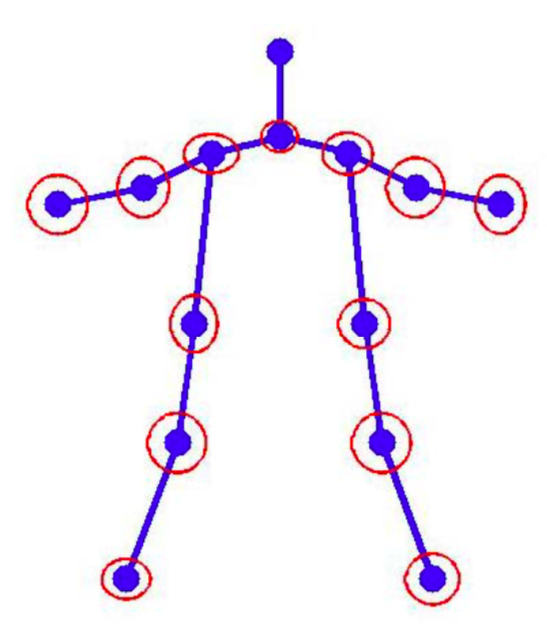
\includegraphics[width=0.35\textwidth]{yang-tree.png}
    \caption{Visualisation of the graph resulting from connecting the joint positions, which form the vertices, together into a human skeleton. Image taken from \cite{yang_articulated_2011}.}
    \label{fig:yang-tree}
\end{figure}

Second, the orientation of a part $i$ is considered relative to its parent part $j$.
For instance, consider the relative position of the part corresponding to \textit{neck} to its parent part \textit{head}.
Necks tend to be below heads (when considering upright people).
The authors use all relative positions found by iterating the dataset and cluster the relative positions into $T=4$ clusters.
The cluster that the part $i$ is put in then defines the type label $t_i$.
See \fref{fig:yang-clustering} for an example.
This then results in a fully annotated dataset with location information $l_i$ as well as type $t_i$ for each part $i$.

\begin{figure}[htb!]
    \centering
    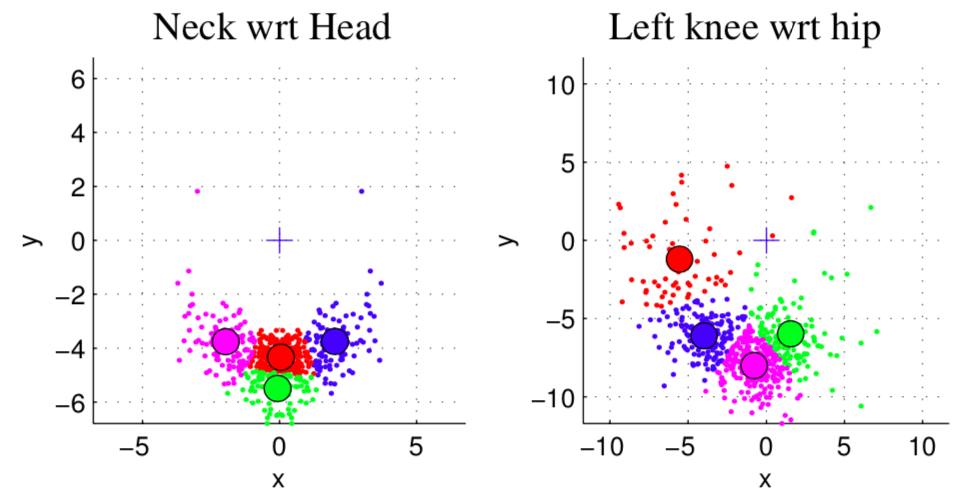
\includegraphics[width=0.65\textwidth]{yang-clustering.png}
    \caption{The relative positions of \textit{neck} with regard to     its parent \textit{head} (\textbf{left}) and \textit{left knee} with regard to \textit{hip} (\textbf{right}). The origin marks the location of the parent. Notice that the neck is generally placed below the head (since most images contain upright people) while the left knee is mostly placed left of the hip. Each color indicates a cluster and a thus a corresponding type label. Image taken from \cite{yang_articulated_2011}.}
    \label{fig:yang-clustering}
\end{figure}

Instead of using one \textit{template} for each limb, the authors propose to use many small templates per limb.
Each template can be of a specific type $t_i$, which can encode semantic features, e.g., open versus closed hand, or orientational information.

%% Score function
The authors provide the following score function to evaluate a predicted pose:

\begin{equation}
    \label{eq:yang-score}
    \begin{split}
        S(I, l, t) 
        &= \sum_{i \in V} b_i^{t_i} + w_i^{t_i} \cdot \phi(I, l_i) \\
        &+ \sum_{(i,j) \in E} b_{ij}^{t_i, t_j} + w_{ij}^{t_i, t_j} \cdot \psi(l_i - l_j)
    \end{split}
\end{equation}

In \eref{eq:yang-score}, $I$ refers to the image that is evaluated.
$l = (l_1, \cdots, l_k)$ is the configuration containing all part positions while $t = (t_1, \dots, t_k)$ corresponds to the types of parts.
$\phi(I, l_i)$ is a Histogram of Oriented Gradients (HoG) feature vector \cite{dalal_histograms_2005} computed around the part position $l_i$.
$\psi(l_i - l_j) = [(x_i - x_j), (x_i - x_j)^2, (y_i - y_j), (y_i - y_j)^2]^T$ encodes the relative location of part $l_i$ to $l_j$.

$w_i^{t_i}$, $w_{ij}^{t_i, t_j}$ as well as $b_i^{t_i}$ and $b_{ij}^{t_i, t_j}$ are parameters estimated from annotated training data, which encode learned relationships between parts as well as type assignments for each part.
During training, a supervised approach is used where the score for an annotated training image is maximized while utilizing regularisation on the models parameters $\beta = (\bm{w}, \bm{w})$.

% Evaluation

To evaluate their model, the authors use \textit{Percentage of Correct Parts (PCP)}, presented in \sref{sec:andriluka-eval}, to be able to compare it to earlier work.
In addition, they define a new metric, \textit{Probability of Correct Keypoints (PCK))}.
In terms of datasets, they use Buffy and Iterative Image Parsing. 

PCK was designed to improve upon two disadvantages of PCP.
First, the toolkit provided with the Buffy dataset \cite{ferrari_progressive_2008} used a definition of PCP different from the one proposed in the paper, which makes the comparison of PCP values in literature hard because it is unclear which definition was used.
The paper definition was provided in \sref{sec:andriluka-eval}.
The Buffy toolkit defines a part as detected if the distance of the average point of both endpoints is within the threshold to the average of the ground truth endpoints.
Second, foreshortening changes the length of the part, which means that the threshold is dependent upon the amount of foreshortening.
This means that foreshortened parts require more accurate predictions to be considered detected.
PCK requires each test image to have a person bounding box annotation.
Using the bounding box dimensions $(width, height)$, a keypoint is considered detected if the distance between the ground truth and prediction is less than $\alpha \cdot max(width, height)$.
This gives a clear reference point for comparison and makes the metric less susceptible to errors due to foreshortened parts.
The paramter $\alpha$ determmines how strict the meassurement should be.
For the Buffy dataset, the authors set $\alpha = 0.2$, while they chose $\alpha = 0.1$ for the Iterative dataset.
They argue that they relaxed the metric for Buffy since the dataset only contains upper-body poses.

As mentioned earlier, the definition of PCP is not clear since the toolkit implementation and paper definition differ.
Thus, the authors computed two different PCP values for each dataset.
First, they use definition presented in the paper, where the distance of both keypoints need to be smaller than the threshold in order for a part to be defined as detected.
This is referred to as the strict definition.
Second, they use the definition provided by the Buffy toolkit, which is more loose since the averages of the keypoints are more likely to be close to each other than both endpoints of the parts.

Even when considering the strictest definition, the model outperforms the previous approaches, including \cite{andriluka_pictorial_2009} (see \sref{sec:andriluka-eval}), on the Iterative dataset.
The authors achieve an overall PCP score of $61.5\%$, which is significantly larger than the $55.2\%$ achieved by \cite{andriluka_pictorial_2009}.
Most notably, the detection rate of the legs is about $10$ percentage points higher when compared to \cite{andriluka_pictorial_2009}.
Since they also propose a new metric, they provide the PCK metric results as well.
Overall, the accuracy achieved is $72.9\%$, which is higher than the overall PCP value.
The authors argue that this might be due to the fact that foreshortened limbs are not penalized unfairly by PCK. 

When evaluating the upper-body Buffy dataset, the authors model outperforms the previous methods, when considering the loose definition, on overall accuracy.
However, when considering the strict definition, they outperform \cite{andriluka_pictorial_2009} with $83.5\%$ (compared to $73.5\%$, see \sref{sec:andriluka-eval}), but are themselves outperformed by other competitors.
When using PCK, the model achieves an overall accuracy of $72.9\%$, which is also higher than the corresponding PCP score.

The authors also evaluate the effect of the number of mixtures defined as well as the number of parts to detect.
The results can be seen in \fref{fig:yang-results-chart}.
While there is a significant increase in accuracy (in terms of PCK) when increasing the number of parts from $14$ to $26$, the effect decreases when further increasing the number of parts.
When evaluating the number of different types, accuracy increases again when increasing the number of mixtures.
They argue that $26$ parts and $6$ mixtures is a good trade-off when considering both accuracy and runtime.  

\begin{figure}[htb!]
    \centering
    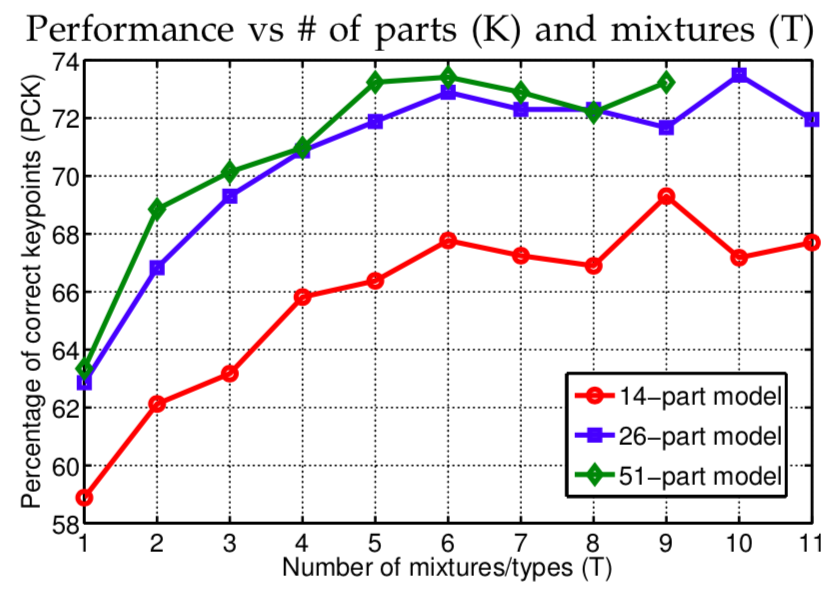
\includegraphics[width=0.5\textwidth]{yang-results-chart.png}
    \caption{The authors find that the higher the number of mixtures ($T$) the higher the accuracy. This is also true, to an extend, with number of parts to detect ($K$). The authors suggest a $26$ part, $6$ mixture model for a good trade-off between accuracy and performance. Image taken from \cite{yang_articulated_2011}.}
    \label{fig:yang-results-chart}
\end{figure}

\subsection{Deep Learning Methods}

\subsubsection{DeepPose}
\label{sec:deeppose}

% Introduction
One of the first approaches for pose estimation using deep convolutional neural networks was proposed by \cite{toshev_deeppose:_2014}.
They achieved state-of-the-art results on two benchmark datasets using a neural network architecture based on the ImageNet network \cite{krizhevsky_imagenet_2012}.
In contrast to the Pictoral Structure framework discussed earlier, the approach was to regress the image coordinates directly without specific prior constrains on how the joints are allowed to be connected.

% Architecture
The authors define their network in terms of multiple connected \textit{stages}.
Each \textit{stage} is comprised of the neural network architecture provied in \tref{tab:deeppose-architecture}.
The only change the authors made from the architecture originally proposed in \cite{krizhevsky_imagenet_2012} was to use the output of the last fully connected layer to regress the joint coordinates as opposed using the softmax activation function.
This means that, assuming $k$ joints should be detected, the output of each stage is of size $2 * k$, because each joint position is given by image coordinates $(x, y)$.
Stage $s_0$ is trained using the full images of size $220 x 220$ as its input.

Once the first stage is trained until convergence, the authors use the output coordinates to crop sub images around the prediction.
By feeding these subimages into the next stage $s_1$ they argue that the predictions of $s_1$ get more precise because local context around the prediction becomes more important.
The sub image size is dependend upon the diameter of the torso bounding box given by the annotations.

This cascading approach is then repeated with the next stages.
In the end, they use $3$ stages $S = (s_0, s_1, s_2)$ after evaluating different numbers of stages on a held-out training set.

\begin{table}[]
    \centering
    \scalebox{0.8}{%
    \begin{tabular}{|l|l|l|l|l|}
    \hline
    \textbf{nr.} & \textbf{layer type} & \textbf{filter size} & \textbf{nr. of filters / neurons} & \textbf{stride} \\ \hline
    1 & convolutional & 11 x 11 x 3 & 96 & 4 \\
    2 & local response normalization &  &  &  \\
    3 & pooling & 3 x 3 &  & 2 \\ \hline
    4 & convolutional & 5 x 5 x 48 & 256 & 1 \\
    5 & local response normalization &  &  &  \\ 
    6 & pooling & 3 x 3 &  & 2 \\ \hline
    7 & convolutional & 3 x 3 x 256 & 384 & 1 \\
    8 & convolutional & 3 x 3 x 192 & 384 & 1 \\
    9 & convolutional & 3 x 3 x 192 & 256 & 1 \\ \hline
    10 & fully connected &  & 4096 &  \\
    11 & fully connected &  & 4096 &  \\ \hline
    12 & fully connected &  & 2k &  \\ \hline
    \end{tabular}}
    \caption{One \textit{stage} of the DeepPose network. Architecture based on \cite{krizhevsky_imagenet_2012}.}
    \label{tab:deeppose-architecture}
\end{table}

% Evaluation
\begin{figure}[htb!]
    \centering
    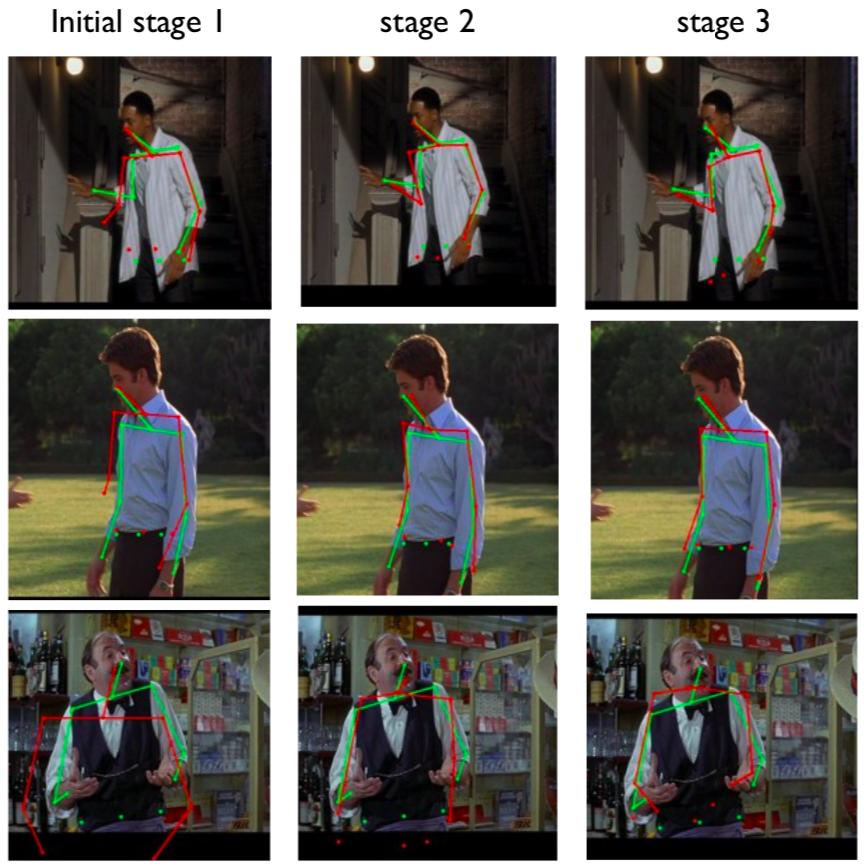
\includegraphics[width=0.5\textwidth]{deeppose-qualitative.png}
    \caption{Qualitative evaluation of the cascading architecture. Ground truth joints are shown in green while predicted poses are shown in red. Notice how the pose gets more accurate with consecutive stages. Also, notice that the biggest improvement can be seen after stage $1$. The authors argue that this is due to the fact that, with an increase in stages, the subimage gets smaller and smaller and thus harder to estimate the pose. Image taken from \cite{toshev_deeppose:_2014}.}
    \label{fig:deeppose-qualitative}
\end{figure}

\label{sec:flic-lsp}
After training their network, the authors evaluate the final model on two datasets, FLIC \cite{sapp_modec:_2013} and LSP \cite{johnson_clustered_2010}.
Frames Labled In Cinema (FLIC) is a dataset which contains $5000$ images of Hollywoord movie scenes where $10$ upper-body joint positions are labeled for the subject of the scene.
In that regard, FLIC is similar to the Buffy dataset.
Leeds Sports Pose (LSP) is a dataset of $2000$ annotated images of subjects in a sport context, which means that the subjects are highly articulated and thus challenging to detect.
LSP contains $14$ different joint positions of the entire body.

The authors use two different metrics to evaluate their model.
First, they use PCP (see \sref{sec:andriluka-eval}) for comparison with the literature.

Also, they define a new metric, \textit{Percentage of Detected Joints (PDJ)}.
They argue, similar to \cite{yang_articulated_2013}, that PCP unfairly penalizes shorter limbs.
With PDJ, a joint is considered detected correctly if the distance between the predicted joint position and the ground truth $d_p$ is smaller than a fraction of the torsos diameter $d_t$.
This fraction is set to be $0.5$, meaning a joint is considered detected if $0 <= d_p <= 0.5 \cdot d_t$.
This metric is similar to PCK in that it compares the distance between two joints to a subject-specific value like torso diameter or subject bounding box.

When comparing the results on the LSP and FLIC datasets, the neural network outperforms the state-of-the-art approaches when considering the PCP metric.
However, like mentioned before, PCP accuracies are hard to compare since there are multiple definitions available.
Thus, the authors reevaluate previous approaches using PDJ and compare their model against these new meassurements.
Again, they outperform the previous state-of-the-art models on both LSP and FLIC.

The authors additionally evaluated their model on the Buffy and Iterative Image Parse datasets, presented in \sref{sec:andriluka-eval}.
This allows a comparison to \cite{yang_articulated_2013}.
Specifically, they trained their model on LSP and evaluated it on Iterative Image Parse for evaluating full-body poses.
Analogously, they train their model on FLIC and evaluate it on the Buffy dataset when considering upper-body poses.

After evaluating on the Iterative Image dataset, they do not share the overall PCP values.
Instead, they compare their results on upper and lower arms as well as upper and lower legs.
These are considered to be the hardest to detect.
On this subset, the model outperforms \cite{yang_articulated_2013} on average by $13$ percentage points ($69\%$ average acccuracy as opposed to $56\%$).

For the Buffy dataset, they do not publish explicit values, but rather the plot in \fref{fig:deeppose-eval}.
From the graphic, it becomes clear that the author's model outperforms \cite{yang_articulated_2013} again, this time in terms of PDJ. 

\begin{figure}[htb!]
    \centering
    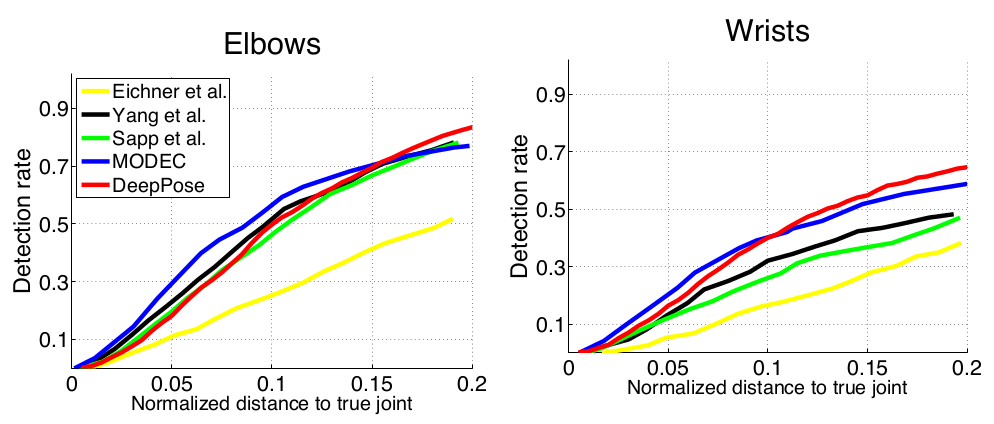
\includegraphics[width=0.8\textwidth]{deeppose-eval-pdj.png}
    \caption{Percentage of Detected Joints for multiple models (elbows and wrists), including \cite{toshev_deeppose:_2014} and \cite{yang_articulated_2013}, on the Buffy dataset. Image taken from \cite{toshev_deeppose:_2014}.}
    \label{fig:deeppose-eval}
\end{figure}

The authors provide three examples which illustrate the importance of the cascading architecture.
These examples can be seen in \fref{fig:deeppose-qualitative}.
They argue that stage $s_1$ has the biggest effect on the accuracy of the joints since further stages use smaller and smaller subimages for regression and thus use a smaller context.
To support their hypothesis, they evaluating three networks in terms of PDJ on the FLIC dataset, with one, two and three stages respectively.
Their findings show the same behaviour observed in \fref{fig:deeppose-qualitative}.

\subsubsection{Convolutional Pose Machine}
\label{sec:convolutional-pose-machine}
% Introduction
Another approach for pose estimation was proposed by \cite{wei_convolutional_2016}.
The authors base their work on \textit{traditional} Pose machines proposed by \cite{ramakrishna_pose_2014}.
In comparison to \cite{toshev_deeppose:_2014}, they do not regress the joint coordinates directly using fully-connected layers but use a fully convolutional architecture to compute \textit{belief maps}.
These maps are very similar to the part evidence maps discussed in \sref{sec:pose-andriluka}, since they indicate the belief of a joint being present at a certain pixel position.

% "Classical" Pose Machine Concepts
Pose machines are a general framework for estimating pose, focusing on refining initial pose predictions based on context from previous decisions.
The modular nature allows to easily use different predictors and encoders, which will be explained in the next section.

The Pose machine is made up of cascaded \textit{stages}.
The first stage uses a predictor $g_1$, which predicts, for each pixel in the input image, how likely it belongs to part $p$.
The result are $P$ belief maps, one for each part to detect.
In all subsequent stages, the output belief maps of the previous stage are encoded back into image features using an encoder function $\varphi$.
Then, these encoded features are combined with the local image features of the current stage and passed into the stage's predictor.
This way, the predictor not only has the image features as a basis for decision but also the previously estimated joint location for context.
See \fref{fig:pose-machines-architecture} for a visualization of the pipeline.

\begin{figure}[htb!]
    \centering
    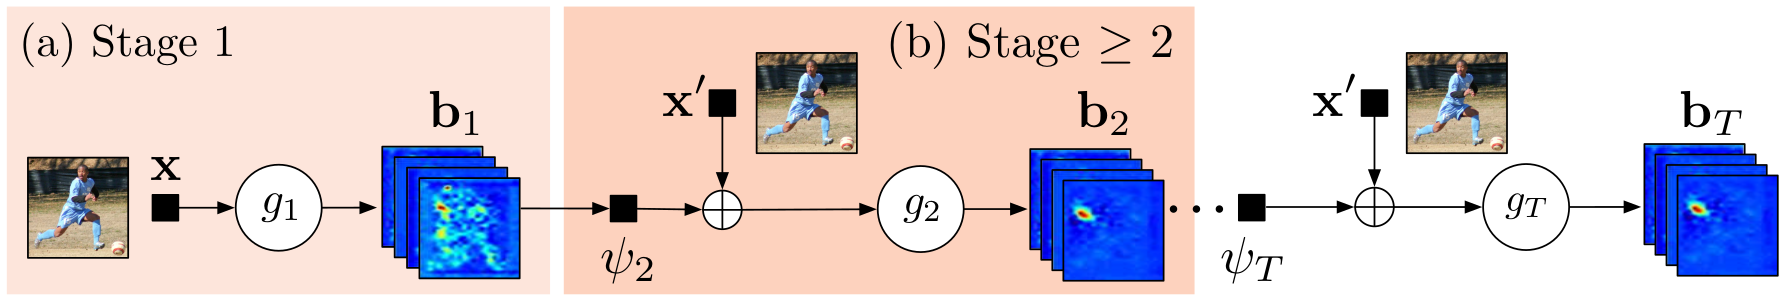
\includegraphics[width=0.9\textwidth]{pose-machine-architecture.png}
    \caption{Cascading stages of the Convolutional Pose Machine. Image taken from \cite{wei_convolutional_2016}.}
    \label{fig:pose-machines-architecture}
\end{figure}

% Concrete Implementation Original
In \cite{ramakrishna_pose_2014}, the authors use boosted random forests for their stage predictors $g_i$.
To extract features, they utilize \textit{Histogram of Oriented Gradients (HoG)} descriptors \cite{dalal_histograms_2005}.
Their encoder $\varphi$ is made up of two parts.
The first part is referred to by the authors as \textit{context patch features}.
For a given pixel coordinate $z = (x, y)$ for each belief map, the authors concatenate the belief scores in a $5 x 5$ grid around $z$.
Afterwards, the concatenated scores from each belief map are again concatenated across belief maps into a final feature vector $\varphi_1$.
The second part, which the authors refer to as \textit{context offset features}, again iterates over all pixel locations $z$.
Given the pixel location of the $3$ highest peaks in the belief map, the feature vector is given by concatenating the relative position to these peaks, given $z$, in polar coordinates.
Again, they concatenate all feature vectors over all belief maps, resulting in $\varphi_2$.
Finally, their context feature vector is given by $\varphi = [\varphi_1, \varphi_2]$.
See \fref{fig:pose-machines-context} for a visualization of $\varphi_1$ and $\varphi_2$.

\begin{figure}[htb!]
    \centering
    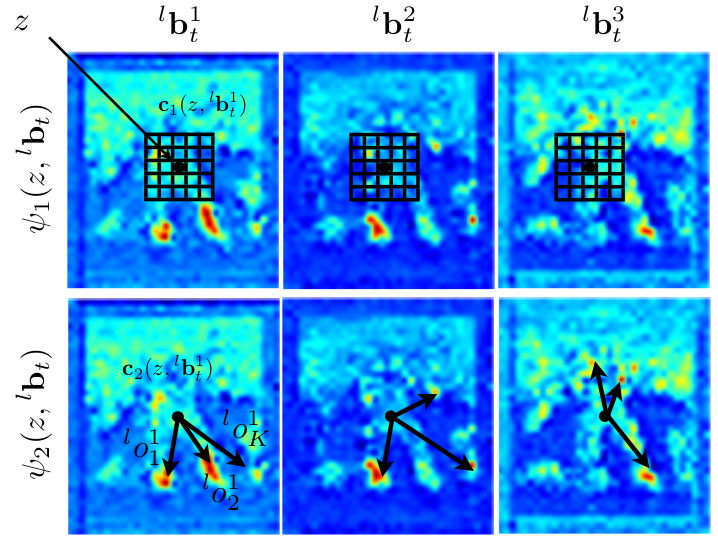
\includegraphics[width=0.6\textwidth]{pose-machine-context-vector.png}
    \caption{Example of context feature extraction, as proposed by \cite{ramakrishna_pose_2014}, for three belief maps $\prescript{l}{}{b_t^1}$, $\prescript{l}{}{b_t^2}$ and $\prescript{l}{}{b_t^3}$ (columns). \textbf{Top row:} Extraction from scores in a $5 x 5$ grid around the pixel $z$. \textbf{Bottom row:} Each arrow points towards one of the top $3$ peaks in the belief map. The polar coordinates with regards to $z$ are then concatenated into the feature vector. Image taken from \cite{ramakrishna_pose_2014}.}
    \label{fig:pose-machines-context}
\end{figure}


% Implementation Convolutional and Differences
In \cite{wei_convolutional_2016}, the authors used convolutional neural networks for their predictors $g_i$.
In fact, the complete architecture is a fully convolutional neural network, allowing end-to-end training of both the decoder and predictor.
Each stage consists of a feature extraction network, of which the architecture is presented in \tref{tab:pose-machine-feature-extraction-architecture} (layers $1$ to $7$).
This leads to the following formulation for the output belief maps $\bm{b}_1$:

\begin{equation}
    \bm{b}_1 = g_1 (x)
\end{equation}

For context encoder $\varphi$, the authors first compute the receptive field size of the previous stage.
Then, when computing the context of position $z = (x, y)$, they center a  window of that size around $z$ in the belief maps.
This leads to 

\begin{equation}
    \bm{b}_t = g_t(x_z, \varphi_t(z, \bm{b}_{t-1}))
\end{equation}

as the output belief maps of stage $t$ with $t > 1$.

The layers in \tref{tab:pose-machine-feature-extraction-architecture} denoted with $a_1$ to $a_3$ refer to the layers after the feature extraction network in the first stage $s_1$.
Analogously, $b_1$ to $b_5$ refer to the layers after the feature extraction network in all subsequent stages $s_i, i > 1$.
The architecture of the first stage, compared to all subsequent stages, differs because the authors want the first stage to have a lower receptive field in order for a more precise extraction of local features.
In fact, the design was chosen so that, after the second stage, the receptive field of the network is roughly the size of the input image.
The authors claim that, through experimentation, this provided the best overall accuracy.

\begin{table}[]
    \centering
    \scalebox{0.7}{%
    \begin{tabular}{|l|l|l|}
    \hline
    \textbf{nr.} & \textbf{layer type} & \textbf{filter size} \\ \hline
    1 & convolutional & 9 x 9 \\
    2 & pooling & 2 x 2\\
    3 & convolutional & 9 x 9 \\
    4 & pooling & 2 x 2\\
    5 & convolutional & 9 x 9 \\
    6 & pooling & 2 x 2 \\
    7 & convolutional & 5 x 5 \\ \hline 
    $a_1$ & convolutional & 9 x 9 \\  
    $a_2$ & convolutional & 1 x 1 \\  
    $a_3$ & convolutional & 1 x 1 \\ \hline 
    $b_1$ & convolutional & 11 x 11 \\  
    $b_2$ & convolutional & 11 x 11 \\  
    $b_3$ & convolutional & 11 x 11 \\ 
    $b_4$ & convolutional & 1 x 1 \\  
    $b_5$ & convolutional & 1 x 1 \\ \hline     
    \end{tabular}}
    \caption{Network architecture of the Convolutional Pose Machine. Layers $1$ to $7$ refer to the feature extraction subnet, which is identical (in terms of architecture) in each stage. However, stages $t > 1$ share the weights of the feature extraction layer to to share the computed image features across stages. $a_1$ to $a_3$ are layers attached to the feature extraction subnet in the first stage, while $b_1$ to $b_5$ are layeres attached to the feature extraction subnet in all subsequent stages.}
    \label{tab:pose-machine-feature-extraction-architecture}
\end{table}

% Number of stages
The authors evaluated the amount of stages to use.
They found that, after $5$ stages, the performance of the network stops increasing, which is why they chose to use $5$ stages for all subsequent experiments.

% Why contexts are helpful
To illustrate why context belief maps can help the network to correct itself, the authors provide the visualization in \fref{fig:context-belief-maps}.
They argue that, even when the belief maps after the first stage are noisy, they can provide useful context information since not every joint is equally hard to detect.
As an example, they argue that \textit{head} and \textit{neck} joints are easier to detect than other joints.
Instead of \textit{right elbow} and \textit{left elbow}, where there are two very similar joints in each image, \textit{head} and \textit{neck} are only present once.
Thus, their position in the first stage belief maps can aid in finding more difficult joints like \textit{right shoulder}.
Similarly, the lack of context information can also help in lessening the score in the belief maps.
For example, consider the local information around \textit{right shoulder}.
Normally, necks and shoulders are near to each other.
When there is no indication of \textit{neck} in the belief map around \textit{right shoulder} this may lead to a lower belief score of \textit{right shoulder} being present at that pixel. 

\begin{figure}[htb!]
    \centering
    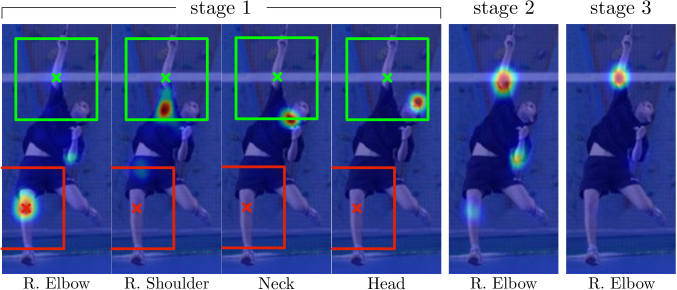
\includegraphics[width=0.8\textwidth]{context-belief-maps.png}
    \caption{Visualization of how context information helps in detecting joint positions. The task at hand is to to find \textit{right elbow}. The current belief map for \textit{right elbow} in stage $1$ is given in the left most image. In green, the authors visualized the receptive field around the ground truth coordinates for \textit{right elbow}, while red illustrates the receptive field around the wrongfully detected joint. Notice that other, easier to detect joints such as \textit{neck} and \textit{head} fall inside the receptive field of the ground truth, suggesting that their positional information can help in locating \textit{right elbow} in further stages due to the context information they provide. The right most two images show the result after the next two stages, where the network corrected itself successfully. Image taken from \cite{wei_convolutional_2016}.}
    \label{fig:context-belief-maps}
\end{figure}

% Evaluation
\label{sec:pose-machine-evaluation}

The authors evaluate their model using three widely used benchmark datasets.
These are LSP and FLIC \sref{sec:flic-lsp} as well as \textit{MPII Human Pose}.  
MPII Human Pose is a benchmark, which consists of $40,000$ annotated images of people.
These images are also often referred to as \textit{in-the-wild} images since they were downloaded from YouTube videos and are thus representative of every day activaties and situations.
In addition, since most YouTube videos are uploaded by private individuals, the image quality varies, making the benchmark more realisitic.
For a complete overview of the MPII dataset, please refer to \sref{sec:exp-mpii}.

For evaluating their model, the authors use both PCK \sref{sec:andriluka-eval} and PCKh metrics.
\textit{PCKh} is used as the metric for the MPII dataset, which is very similar to both PCK and PDJ \sref{sec:flic-lsp}.
However, instead of using the person bounding box or torso bounding box for normalization, PCKh uses the head bounding box.
\cite{andriluka_2d_2014} argue that PCKh is more useful for evaluating highly articulated poses compared to PCK since the full body bounding box can be fairly large for some poses.
Consider a person, jumping in the air, spreading their arms and legs away from their body.
This maximizes the person bounding box and thus makes it easier for the PCK metric to consider predictions to be correct when they are fairly far away from the ground truth.
The head size, aswell as torso size, however, is quite independent from the type of pose and thus more suitable for evaluation.
In addition, they use PCK in order to compare their results on FLIC and LSP to the literature.

When evaluating their model using the LSP dataset, they found that, using a six stage model, they outperform the state-of-the-art approaches by approximately $15$ percentage points.
The improvement is especially noticeable when evaluating the challenging joints like ankles.
The result got even better ($~20$ percentage points increase) when utilizing additional training data from the MPII dataset.
The authors argue that this is due to the fact that the LSP datasets contains noisy annotations when compared to the annotations provided by MPII.

Afterwards, the authors compare their results on the FLIC dataset to many state-of-the-art models, including \cite{toshev_deeppose:_2014} \sref{sec:deeppose}.
They compare their result on two challenging type of joints, namely wrists and elbows.
Again, they outperform all state-of-the-art approaches.
When comparing their results specifically with \cite{toshev_deeppose:_2014} the authors outperform their result by approximately $15$ percentage points for wrists and approximately $9$ percentage points for elbows.
Also, in contrast to their LSP evaluation, they did not incorporate training data from MPII.

% Evaluate against traditional Pose Machine
When comparing their results with the traditional Pose machine, they find that the convolutional approach improves upon the results on the LSP dataset by an overall PCK accuracy improvement of $42.4$ percentage points.

% Intermediate supervision and connection to vanishing gradient

\begin{figure}[htb!]
    \centering
    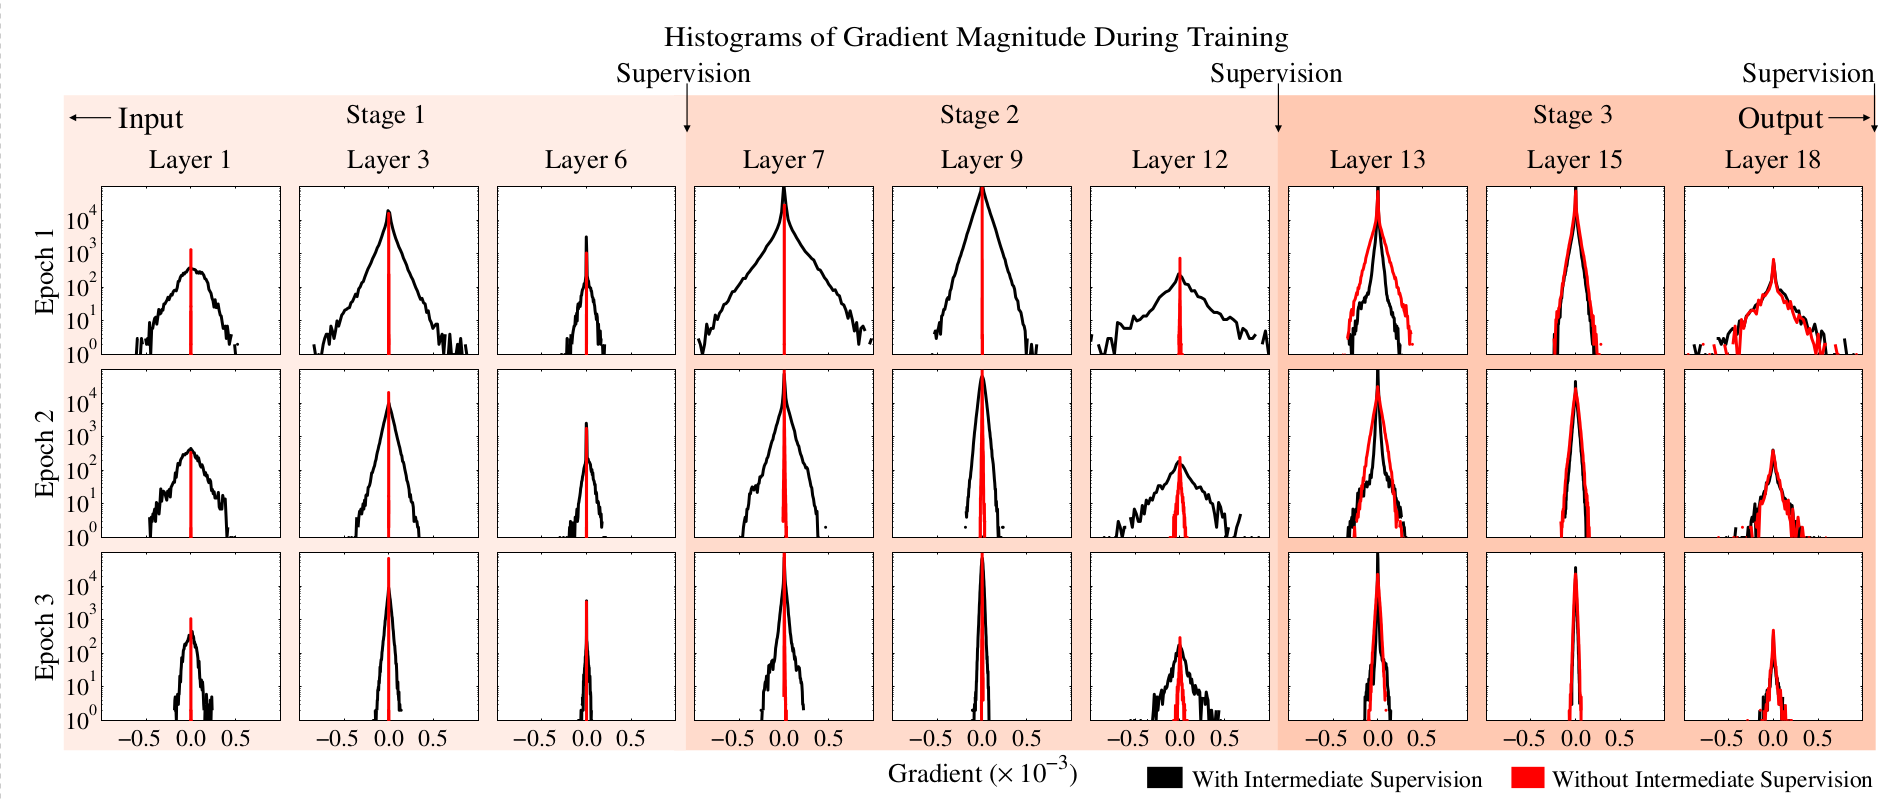
\includegraphics[width=0.99\textwidth]{posemachine-vanishing-gradient.png}
    \caption{Gradient magnitude and variance across some layers of the Convolutional Pose Machine. When not using intermediate supervision (\textbf{red}), the gradient variance approaches zero towards the beginning of the network, effectively stopping the learning process.  When using intermediate supervision, however, notice that the variance of the gradients generally does not approach zero. Image taken from \cite{wei_convolutional_2016}.}
    \label{fig:pose-machine-vanishing-gradient}
\end{figure}

The authors also evaluated the result of intermediate supervision on the vanishing gradient problem \sref{sec:vanishing-gradient}. 
They trained two networks, one with intermediate supervision and one without, for the same amount of time.
Their results are visualized in \fref{fig:pose-machine-vanishing-gradient}.
The authors argue that the reason why intermediate supervision does help against the vanishing gradient problem is because it replenishes the gradient after each stage and thus keeps the gradient from decreasing when propagating back towards the network.

\subsubsection{Stacked Hourglass}
\label{sec:stacked_hourglass}
% Introduction
Building on \cite{toshev_deeppose:_2014}, \cite{newell_stacked_2016} proposed the \textit{Stacked hourglass network}.
Similar to \cite{wei_convolutional_2016}, the authors compute \textit{belief maps} encoding joint probabilities instead of regressing the coordinates directly.
However, the authors refer to them as \textit{heatmaps}.

Similar to the previously discussed approaches for convolutional architectures, the authors use a stacked architecture, where predictions get refined iteratively.
They do, however, not crop the input down with each iterative step like \cite{toshev_deeppose:_2014} but keep the whole image in every step (similar to \cite{wei_convolutional_2016}).
The authors argue that refinement of joint positions inside a local subimage is not optimal since many errors occur when misattributing joint positions.
Thus, limiting the network to local images might hinder its ability to make big changes in joint positions.

\begin{figure}[htb!]
    \centering
    \includegraphics[width=0.8\textwidth]{stackedhourglass.png}
    \caption{Schematic visualization of the stacked hourglass network. Notice the hourglass-shaped symmetric submodels connected together. Image taken from \cite{newell_stacked_2016}. }
    \label{fig:stacked-hg-architecture}
\end{figure}

% Architecture
The building blocks of the stacked hourglass archtitecture are so-called \textit{hourglass modules}.
See \fref{fig:single-hourglass} for a visualization of a single hourglass module.
The idea is to process the input of the module at different scales and then combine features from different scales using \textit{skip-connections}.

\begin{figure}[htb!]
    \centering
    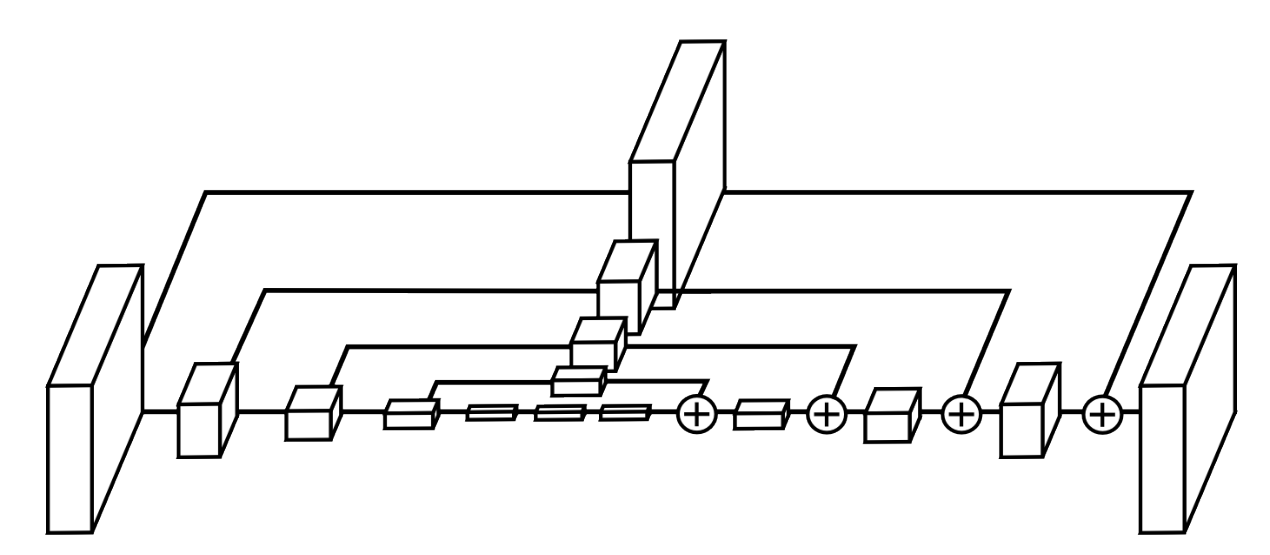
\includegraphics[width=0.6\textwidth]{single-hourglass.png}
    \caption{Visualization of a single hourglass module. Each block is a residual module, consisting of multiple convolutional layers with skip-connections. Notice how the skip-connections combine features at different scale levels. Image taken from \cite{newell_stacked_2016}. }
    \label{fig:single-hourglass}
\end{figure}

A skip-connection is a path in the network, which branches of at a certain point and gets combined with the original path again further down the network.
For example, consider a neural network with three convolutional layers.
A skip-connection could branch of before the first convolutional layer, apply some processing in forms of additional convolutional layers, and get added back into the original path after the second convolutional layer, thus effectively \textit{skipping} the processing of the first and second convolutional layers.
Thus, earlier features (in terms of network depth) can be reintroduced at a later stage and long-range dependencies between variables can be modelled.
One common use-case for skip-connections, which the authors used, is to reintroduce lower level features and add them to higher level features.
This way, tasks like pose estimation can incorporate global, high level features like body shape with low level, local features like faces.

\label{sec:residual_blocks}
Skip-connections get used in \textit{residual blocks} \cite{he_deep_2016}, which are used for more efficient learning in deep networks.
Consider two connected convolutional layer with input $x$.
Let $f(x)$ be the output of the second convolutional layer.
Residual models model $f(x) + x$ because they use the skip-connection to add the input back to the output.
The authors of \cite{he_deep_2016} argue that this allows for deeper neural network architectures because it is easier to fit identity mappings.
They evaluated deep neural networks and found that the error does not only not decrease for very deep networks but starts increasing.
The authors argue that this would not happen if the layers would learn identity functions because then the error would stagnate instead of increase.
In addition, because residual blocks allow for very deep architectures, they achieved substantially better results in comparison to identical architectures without residual blocks.

An example of a residual blocks used in the stacked hourglass network can be seen in \fref{fig:hg-residual}.
In fact, all blocks shown in \fref{fig:single-hourglass} are residual blocks.

\begin{figure}[htb!]
    \centering
    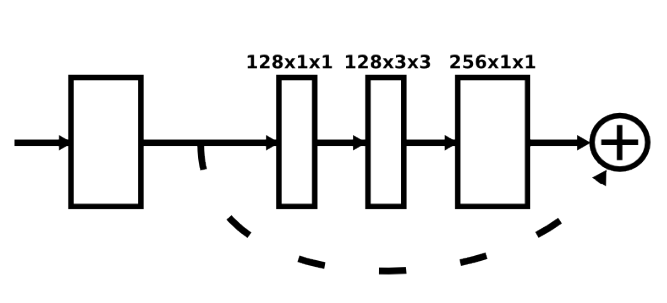
\includegraphics[width=0.4\textwidth]{residualmodule.png}
    \caption{A residual module \cite{he_deep_2016}, as used in the stacked hourglass network. The module is made up of a batch normalization layer (left) and three convolutional layers, each utilizing the ReLU activation function. The dotted line visualizes the skip-connection. Image taken from \cite{newell_stacked_2016}. }
    \label{fig:hg-residual}
\end{figure}

Each hourglass module is a network with a symmetrical architecture.
For each downsampling step with a pooling layer there exists a corresponding upsampling step using \textit{nearest-neighbour upsampling}.
% TODO: One sentence explain
Consequently, the input and output dimensions of the hourglass module are identical, allowing multiple modules to be applied one after the other.

The input to the module is scaled down using pooling layers, until it reaches a resolution of $4x4$ pixels.
At each resolution level, features are extracted using a residual module.
Before each pooling layer, a skip-connection is utilized to branch off the current feature maps.
They get feed through another residual block and combined back later.
Once image is scaled down to $4x4$ pixels, upsampling is utilized until the image is back to its original size.
Again, residual blocks are used to extract features at the different levels of resolution.
Also, after the feature extraction, the processed skip-connections from earlier get added onto the extracted features, effectively combining features from two different image scales, because they get combined before upsampling happens.

The authors use another skip-connection between the input and output of the module.
This means that the input to each module, which is the output of the previous module, is added onto its output.
The authors argue that this allows the network to refine its prediction with each hourglass module since the high level features, which are the outputs of each module, get processed by consecutive hourglass modules again, creating higher order spatial relationships.

They qualitatively observe that errors made by early modules can be corrected by later modules.
Also, they evaluated the difference between $2, 4$ and $8$ stacked hourglasses, which will be referred to as $s_2, s_4$ and $s_8$.
For a better comparability, they altered the hourglass archictecture for the $s_2$ and $s_4$ to keep the number of trainable parameters the same between architectures.
For each residual block in each hourglass in $s_2$ the authors substituted $4$ residual blocks, effectively quadrupeling the number of residual blocks.
Analogously, they doubled the amount of residual blocks for $s_4$.
When training $s_2, s_4$ and $s_8$, they found validation accuracies of $87.4\%$, $87.8\%$ and $88.1\%$ respectively, suggesting that the stacked architecture does contribute to higher overall accuracies.
In the final architecture, the authors use $8$ hourglass modules.

While training, the output of each hourglass module is not only feed into the next module, but also processed into a \textit{heatmap} using a $1x1$ convolutional layer.
Using this heatmap, a loss is computed after each hourglass module, which is then propagated back.
The authors refer to this process as \textit{intermediate supervision} and argue that it increases the accuracy of the final prediction because the network needs to develop a high-level of understanding very early.
In their quantitative analysis, they showed an increase in validation accuracy of around $3$ percent when utilizing intermediate supervision. 

% Evalutation
%% Meassurements and Datasets
For evaluating the stacked archictecture, the authors used the \textit{FLIC} \sref{sec:flic-lsp} and \textit{MPII Human Pose} \cite{andriluka_2d_2014} datasets.

In terms of metrics, the authors take the same approach as \cite{wei_convolutional_2016}, where they use PCKh for MPII Human Pose and PCK for FLIC.
For \textit{FLIC}, they defined $\alpha = 0.2$, which means that $20\%$ of the length of the head is used as the threshold.
They compare their results to \cite{toshev_deeppose:_2014} and outperform their results on elbows and wrists by $6.7$ percentage points ($99.0\%$ compared to $92.6\%$) and $15$ percentage points ($97\%$ compared to $82\%$), respectively.
In addition, they outperformed \cite{wei_convolutional_2016}, the state-of-the-art appraoch at that time \sref{sec:convolutional-pose-machine}.

With \textit{MPII Human Pose}, the threshold was reduced to $50\%$ in accordance to the previous works they compared against.
Also, PCKh was used instead of PCK, as described before, since PCKh was proposed in \cite{andriluka_2d_2014}, and thus most models using the MPII dataset use PCKh for evaluation.
Similar to before, they outperformed the state-of-the-art approaches, including \cite{wei_convolutional_2016}.
In particular, they achieved $90.9\%$ overall accuracy as compared to $88.5\%$ achieved by \cite{wei_convolutional_2016}.
Also, they achieved significantly better results on each individual part, including a $3.5$ percentage point increase on the average over the most challenging joints (wrists, elbows, kness and ankles) in comparison to \cite{wei_convolutional_2016}. 

% \begin{itemize}
%     \item Cascade Feature Aggregation for Human Pose Estimation \cite{su_cascade_2019}
% \end{itemize}

\section{Video-based Human Action Recognition}

In the following chapter, approaches for Human Action Recognition on video data will be discussed.
First, some prominent works utilizing hand-crafted features will be discussed.
These approaches still perform well in modern scenarios and are sometimes used in conjunction with modern, neural network based approaches.
Second, the Two-Stream architecture will be discussed, as it is the foundation for many state-of-the-art approaches today.
Finally, Human Action Recognition approaches explicitly utilizing pose feature information are presented, since they show promise for end-to-end learning of the Human Action Recognition pipeline by training the pose estimator in tandem with the action classification network. 

\subsection{Shallow Methods}
\label{sec:har_shallow}
\subsubsection{Learning realistic human actions from movies}
\label{sec:laptev-shallow}

% Intro
For a long time, action recognition research focused on simple video datasets such as KTH \cite{schuldt_recognizing_2004}, which feature a small number of different actions, recorded in simple environments like laboratories.
While important for the initial research into the methodology, such datasets do not represent real world scenarios and are thus not ideal when deciding whether an algorithm performs well in the real world.

The authors of \cite{laptev_learning_2008} gathered a novel dataset, which will be referred to as the \textit{Hollywood1} dataset.
This dataset was gathered from movie scenes, which are close to real world scenarios in the sense that they have diverse backgrounds, feature occlusion pf the subject by other entities in the scene as well as differences in clothing, overall making the action recognition process more challenging than in previous datasets.

The dataset contains eight different actions, \textit{Answer Phone, Get Out Of Car, Handshake, Hug Person, Kiss, Sit Down, Sit Up} and \textit{Stand Up}, which were gathered from $12$ movies for the training and from $21$ different movies for the test set, resulting in $219$ and $211$ clips respectively.

% 2D Harris Corner
In addition to the new dataset, the authors also propose a novel approach for action recognition, building on the work of \cite{laptev_harris3d}, where the Harris corner detector is expanded to also detect interest points in the temporal dimension, making it suitable for action recognition in videos.

The Harris corner detector \cite{harris_combined_1988} finds corners, also referred to in the literature as \textit{interest points}, by finding locations where the image expresses significant changes of intensity in both $x$ and $y$ direction \cite{laptev_harris3d}.
By using a small window $W$, which is moved over the image $I$, and displacing the content of the window, an error term can be computed to the original, non-displaced image patch, using the following formula:

\begin{equation}
    f(\Delta x, \Delta y) = \sum_{x_i, y_i \in W} (I(x_i,y_i) - I(x_i + \Delta x, y_i + \Delta y))^2.
\end{equation}

By using the Taylor series to approximate the second term of the subtraction, the error formula simplifies to

\begin{equation}
    \begin{split}
        f(\Delta x, \Delta y) 
        &\approx \sum_{x_i, y_i \in W} (I_x(x_i, y_i) \Delta x + I_y(x_i, y_i) \Delta y)^2 \\
        &\approx (\Delta x, \Delta y) M \binom{\Delta x}{\Delta y}.
    \end{split}
\end{equation}

$
M = \sum_{x_i, y_i \in W} 
\begin{bmatrix}
    I_x^2 & I_x I_y \\
    I_x I_y & I_y^2
\end{bmatrix}
$ is the second-moment matrix, with $I_x, I_y$ being the partial derivatives of $I$ in $x$ and $y$ direction, respectively.
According to \cite{laptev_harris3d}, $M$ can be interpreted to describe the covariances around the window center.
Using the eigenvalues $\lambda_1, \lambda_2$ of $M$, edges and corners can be detected in the following way.
If $\lambda_1 >>\lambda_2$ or $\lambda_1 << \lambda_2$, then an edge has been detected, since large change is only detected in one direction.
Similarly, if both eigenvalues are small, then very little change is detected in both directions, meaning that the patch does neither contain an edge nor a corner.
However, if both eigenvalues are sufficiently large, a corner is detected, since significant change in both directions was observed.

% Extension to 3D
To detect these interest points in a spatio-temporal context, \cite{laptev_harris3d} extended the Harris corner detector to three dimensions.
This means that the image sequence needs to express high changes in $x$, $y$ and the temporal direction $t$.
The first change is the dimension of $M$, which is now a $3 \times 3$ matrix, given by the following formula:

\begin{equation}
    M_3 = \sum_{x_i, y_i, t_i \in W} 
    \begin{bmatrix}
        I_x^2 & I_x I_y & I_x I_t \\
        I_x I_y & I_y^2 & I_y I_t \\
        I_x I_t & I_y I_t & I_t^2
    \end{bmatrix}.
\end{equation}

This in turn results in three eigenvalues $\lambda_1, \lambda_2$ and $\lambda_3$, which can then be used as discussed previously to detect interest points.
An example of detected spatio-temporal interest points are shown in \fref{fig:spatio-temporal-interestpoints}.

% Method
\begin{figure}[htb!]
    \centering
    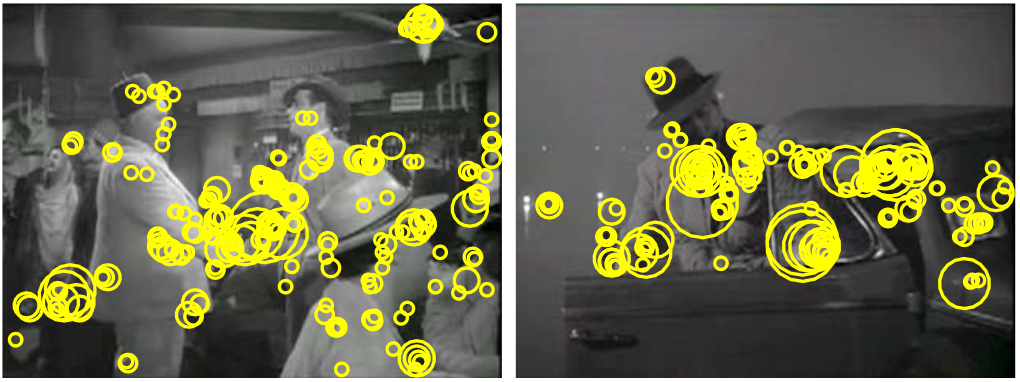
\includegraphics[width=0.7\textwidth]{spacetimeinterestpoints.png}
    \caption{Two examples of spatio-temporal interest points calculated on move frames. \textbf{Left}: Scene of two people shaking hands. Notice the cluster of interest points around the subjects hands. \textbf{Right}: A person gets out of the car. Again, notice the cluster forming around the car door as well as the person performing the action. Image taken from \cite{laptev_learning_2008}. }
    \label{fig:spatio-temporal-interestpoints}
\end{figure}

Using the computed spatio-temporal interest points, the authors proceed to extract image descriptors around them.
First, they define a volume around each interest point, the size of which is dependent upon the image scale since they compute features for multiple scales of the original image.
Each of those volumes is then further partitioned into subvolumes of size $3 \times 3 \times 2$, where $2$ refers to the number of consecutive frames.
On each of those subvolumes, the authors compute \textit{Histogram of Oriented Gradients (HoG)} as well as \textit{Histogram of Oriented Flow (HoF)} descriptors.
Similar to HoG, Histogram of Oriented Flow discretises and clusters the values of a optical flow image into bins.
Then, a histogram is created, containing the number of items for each bin.
The authors, however, do not mention which algorithm was used to compute the optical flow.
The histograms of all subvolumes are first normalized and then concatenated, resulting in a single HoG and HoF descriptor per volume.

Before classification, the authors utilize the bag-of-features approach to cluster the computed image descriptors.
They take $100,000$ random features computed earlier and cluster them into $4,000$ clusters using the k-Means algorithm \cite{macqueen_methods_1967}\cite{lloyd_least_1982}.
The number of clusters was chosen because the authors claim that, empirically, this leads to good results.

\begin{figure}[htb!]
    \centering
    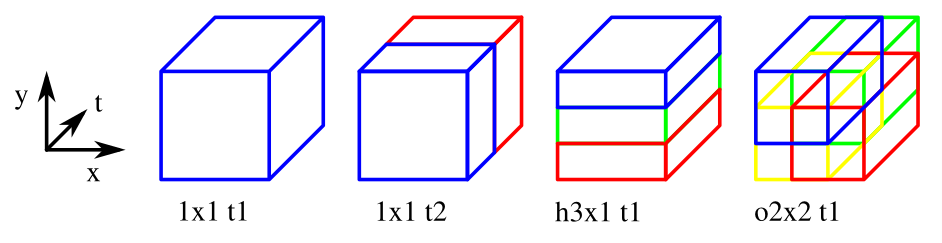
\includegraphics[width=0.7\textwidth]{spatio-temporal-grid.png}
    \caption{Four examples of spatio-temporal grid evaluated by the authors. \textbf{From left to right}: \textbf{(1)} Using the whole clip to compute the histogram. , \textbf{(2)} Split the number of frames in half, compute separate histograms and concatenate afterwards, \textbf{(3)} Split the clip horizontally into three subvolumes, spanning the whole temporal dimension, \textbf{(4)} Choose overlapping subvolumes in the spatial dimensions. The authors found \textbf{(3)} to achieve the best results. Image taken from \cite{laptev_learning_2008}. }
    \label{fig:spatio-temporal-grid}
\end{figure}

To compute the descriptor for a video clip, the authors divide the whole volume of the clip into three horizontal subvolumes.
They refer to this as the spatio-temporal grid.
For each subvolume, the descriptors computed are assigned to the nearest of the $4,000$ cluster centers and a histogram is computed over the cluster centers.
Finally, the histograms of all subvolumes are concatenated and normalized, resulting in the final descriptor of the video clip.
The authors evaluated different methods of subdividing the video clip and found the approach using three horizontal subvolumes to perform the best.
They argue that this is due to the nature of the dataset, where (mostly upright) subjects perform actions, and thus distinctions in horizontal direction are more important than in vertical direction.
See \fref{fig:spatio-temporal-grid} for a visualization of some spatio-temporal grids evaluated by the authors.
The grid described above is shown at position \textbf{(3)}.
% TODO: ? Done on multiple scales $\sigma$, $\tau$. ?

% Evaluation
First, the authors compare their approach to the state-of-the-art approaches on the KTH benchmark \cite{schuldt_recognizing_2004}.
This dataset contains the classes \textit{Walking, Jogging, Running, Boxing, Waving} and \textit{Clapping}.
The video sequences are recorded in front of mostly uniform backgrounds such as white walls or on grass.
The authors achieve an increase in accuracy of $5.1$ percentage points over the previous best approach by \cite{wong_extracting_2007}.
The classes which the authors approach wrongly classified the most were \textit{Jogging} and \textit{Running}, which are very similar actions.
When evaluating their approach on the \textit{Hollywood1} dataset, they report average precision values of $18.2$ percent for the worst class (\textit{Sit Up}) and $53.3$ percent for the most accurate class (\textit{Kiss}).
Overall, their approach achieves a mean average precision of $38.38$ percent.

\subsubsection{Dense Trajectories}
\label{sec:dense-trajectories}

Similar to \cite{laptev_learning_2008}, many approaches in the action recognition literature focused on creating spatio-temporal descriptors, often based on known 2D descriptors like 3D-SIFT \cite{scovanner_3d_sift} and HOG3D \cite{klaser_hog3d}.
However, the authors of \cite{wang_dense_2013} argue that, due to the different characteristics of the spatial and temporal domain, tracking 2D descriptors over time should lead to a higher accuracy in action recognition.
They propose to densely sample points on the first frame of a video clip and then tracking them on trajectories throughout the clip.
Afterwards, image descriptors are computed along these dense trajectories.

\begin{figure}[htb!]
    \centering
    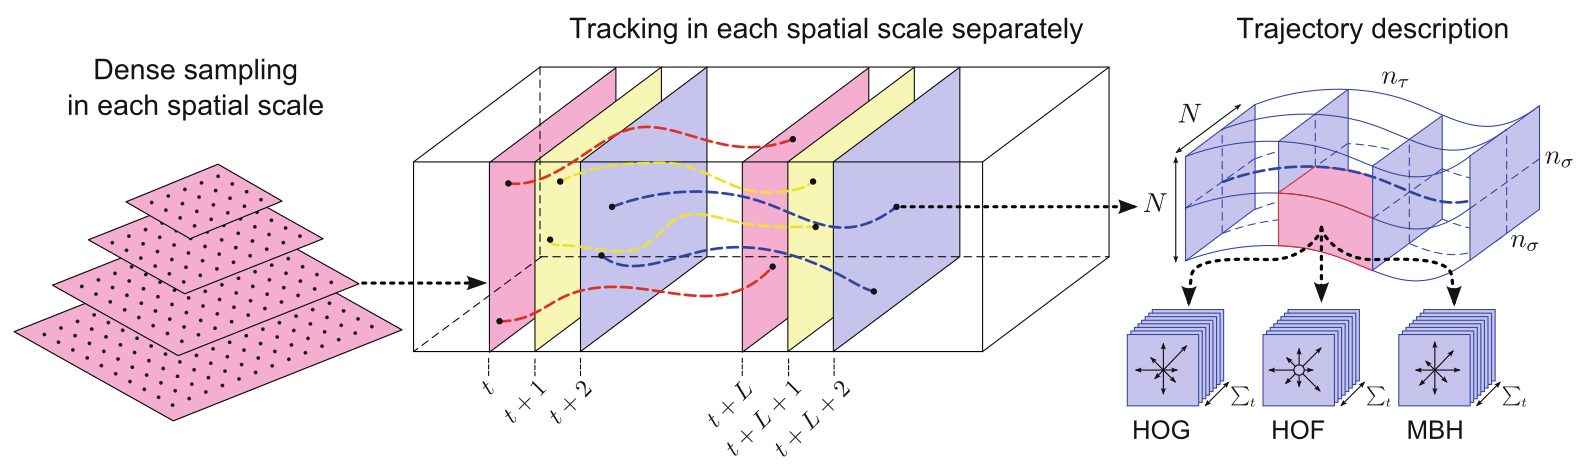
\includegraphics[width=0.9\textwidth]{dense_trajectories_overview.png}
    \caption{Overview of the Dense Trajectories method proposed by \cite{wang_dense_2013}. First, dense interest points are sampled at different scales of the first frame of the video clip. Then, using precomputed optical flow, these points are tracked through the video, resulting in a trajectory. Afterwards, image descriptors are computed along the trajectory. Image taken from \cite{wang_dense_2013}. }
    \label{fig:dense-trajectories-overview}
\end{figure}

% Trajectory
They start by sampling the initial interest points in a $5$ pixel grid.
Afterwards, they decide to prune the grid to reduce the amount of computation necessary.
This is achieved by removing sample points which are located inside homogeneous areas, e.g., walls in the background or other flat surfaces.
This is necessary because reliably tracking points over homogeneous areas using optical flow is impossible \cite{wang_action_2013}.
Also, optical flow is computed on all consecutive frame pairs using the optical flow algorithm provided by the OpenCV library \cite{bradski_opencv_2000}.
Then, they proceed to track each interest point using the optical flow field for $15$ frames, which results in a trajectory $(P_1, P_2, \dots, P_t)$ with $t \in [1, 15]$.
This process is repeated for different scales of the image in order to extract local and global image features.
See \fref{fig:dense-trajectories-overview} for visualization of the process.
The authors argue that limiting the length of a trajectory is necessary in order to avoid the trajectory from drifting away from the initial interest point too much.
In the case where a trajectory is too stationary the authors prune it afterwards because they argue that such a trajectory does not contain sufficient motion information to be useful.
Analogously, in the case where a trajectory contains a jump which is higher than $70$ percent of the overall displacement since the initial interest point the trajectory is also pruned, since, according to the authors, such a large displacement is usually present due to errors.
Also, in the case where an interest point vanishes from one frame to another or a displacement larger than a certain threshold is occurring they decide to start a new trajectory by sampling a new initial point in the area where the last point was.
The authors do not, however, specify how large this threshold is.

% Descriptors
Along each trajectory, the authors compute four different descriptors.
The first descriptor contains the relative motion between consecutive trajectory points $\Delta P_t = (P_{t+1} - P_t) = (x_{t+1} - x_t, y_{t+1} - y_t)$.
This vector is further normalized by the sum over all relative displacements, resulting in the following descriptor $T$ given the length of the trajectory $L$:

\begin{equation}
    T = \frac{(\Delta P_t, \dots, \Delta P_{t + L -1})}{\sum_t^{t+L-1} \lVert \Delta P_t \rVert}
\end{equation}

The authors use \textit{Histogram of Oriented Gradients (HoG)} \cite{dalal_histograms_2005}, \textit{Histogram of Optical Flow (HoF)} \cite{laptev_learning_2008} (see \sref{sec:laptev-shallow} for more information) as well as \textit{Motion Boundary Histograms (MBH)} \cite{dalal_human_2006} to extract features along the trajectories, similar to the approach of \cite{laptev_learning_2008} \sref{sec:laptev-shallow}.
Centered at each interest point along a trajectory, a $N \times N$ pixel area is defined with $N = 32$.
These areas are then again subdivided into $n_\sigma \times n_\sigma$ subareas with $n_\sigma = 2$.
The descriptors are then computed on each of these subareas and descriptors over $n_\tau = 3$ timesteps are then summed to form a single descriptor for each $n_\sigma \times n_\sigma \times n_\tau$ subvolume.
Afterwards, these subvolume descriptors are aggregated, resulting in a single descriptor for each type (HoG, HoF, MBH) and each subvolume $N \times N \times n_\tau$.
See \fref{fig:dense-trajectories-overview} (right) for a visualization of this process.

Motion Boundary Histograms, originally proposed by \cite{dalal_human_2006}, are computed using optical flow between consecutive frames.
First, optical flow for both $x$ and $y$ direction is computed.
Afterwards, gradients are computed on both $x$ and $y$ flow images.
On these gradient images, a histogram is computed analogously to HoG using eight bins.
It is argued that MBH is highly robust to camera motion since this kind of motion is mostly constant in a movie context and thus results in the gradient of the optical flow being close to zero. 
The authors decide to compute separate descriptors for $x$ and $y$, resulting in MBHx and MBHy.
For HoG and HoF, they also chose to use eight bins for quantization.
Additionally, for HoF, a ninth bin is added in cases where the flow magnitude is lower than a not specified threshold.

The authors evaluate the contribution of each of the four descriptor types to the overall accuracy on multiple datasets.
First, they find that the trajectory descriptor using the relative displacement vectors outperforms HoG on datasets where the background is not complex, i.e., in a laboratory environment.
They argue that this is because tracking is significantly easier in such a environment.
On datasets which focus on sport activities, HoG consistently outperforms HoF.
The authors argue that this is due to the importance of spatial context in sports actions since they often involve objects, i.e., a ball or a javelin, and specific environmental scenarios, such as arenas or track fields.
Additionally, the authors find that MBH outperforms all other descriptors on most datasets.
Especially in videos which are recorded by private individuals using cheap cameras or mobile phones MBH gains an advantage over other descriptors because it suppresses camera motion.
In general, according to the authors, using all descriptors in combination for classification yields higher accuracies than only using a subset, suggesting that both temporal and spatial information are necessary for high accuracy.

In addition, they compared their findings against \cite{laptev_learning_2008}, discussed in \sref{sec:laptev-shallow}.
For comparison, they used two datasets.
The \textit{Youtube} dataset \cite{liu_recognizing_2009} contains video clips gathered from the video streaming platform YouTube.
The dataset contains $11$ different actions, mostly from the context of sport.
The other dataset is \textit{Hollywood2} \cite{marszalek_actions_2009}, which is an extension of the previously discussed \textit{Hollywood1} dataset \cite{laptev_learning_2008} (see \sref{sec:laptev-shallow}).
First, the number of actions was increased to $12$ by adding \textit{Fight Person, Run, Eat} and \textit{Drive Car}.
Additionally, the number of training video clips was increased to $810$ while the number of test clips was increased to $884$. 

To accurately compare both approaches, they utilize the interest points computed by \cite{laptev_learning_2008} to compute the HoG and HoF descriptors.
In a direct comparison, both HoG and HoF descriptors on their own lead to the same accuracy regardless of whether the trajectory is used or the interest points computed by \cite{laptev_learning_2008}.
However, the MBH descriptor consistently outperforms both HoG and HoF, and by combining MBH with HoG and HoF the authors achieve a significant accuracy gain of $7.0$ percentage points on the YouTube dataset and $4.2$ percentage points on the Hollywood2 dataset over \cite{laptev_learning_2008} ($76.2$ versus $69.2$ percent and $51.9$ versus $47.7$ percent, respectively).

\subsubsection{Improved Dense Trajectories}
\label{sec:improved-dense-trajectories}
% Intro
After their work in \cite{wang_dense_2013}, some of the same authors improved upon their work in \cite{wang_action_2013}.
The new approach is named \textit{Improved Dense Trajectories (IDT)}.
The core idea is to remove the camera motion before computing the dense trajectories, resulting in a optical flow field which contains less background information.
To achieve this, the authors assume that two consecutive frames can be related to each other using a homography.

% Homography
In general, a homography $H$ relates two points $x$ and $x^\prime$ in the same plane by $x^\prime = Hx$ \cite{vincent_detecting_2001}.
$H$ is defined as a $3 \times 3$ matrix since the image points $x = (x_x, x_y, 1)$ are projections of three dimensional points onto the camera plain.
Also, a homography can express the relationship between the same point but viewed by two different cameras, or, as shown later, a single camera before and after displacement.
Let $F_1, F_2$ be two images, taken by the same camera, but at different world positions.
Using matching points between $F_1$ and $F_2$, $H$ can be computed.
With $H$, the camera movement in $F_2$ can be removed, resulting in a reduction of background movement.
This procedure is further referred to as warping.

\begin{figure}[htb!]
    \centering
    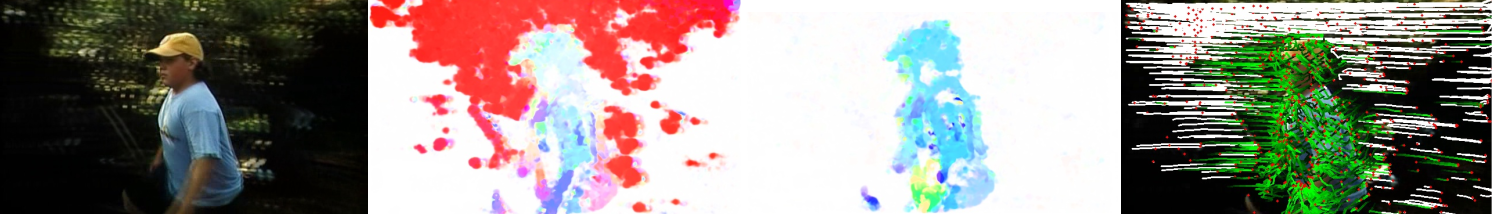
\includegraphics[width=0.99\textwidth]{idt-stages.png}
    \caption{Overview over the different stages of the Improved Dense Trajectories algorithm. \textbf{Outer left}: Two consecutive frames displayed over another. Notice the blurry background. \textbf{Middle left}: Computed optical flow without warping. \textbf{Middle right}: Optical flow computed where the second frame was warped according to the computed homography. Notice that the background motion has vanished and the motion of the subject is much more pronounced. \textbf{Outer right}: Trajectories computed on the warped flow. Background trajectories, which are removed, are displayed in white .Image taken from \cite{wang_action_2013} and modified from vertical stack to horizontal stack. }
    \label{fig:idt-stages}
\end{figure}

The authors argue that the homography assumption, requiring the motion between frames to be planar, holds in their scenarios most of the times since the movement by independent subjects in the frame, such as actors, is small enough to be negligible.
To compute $H$, the authors first compute SURF detectors \cite{bay_surf:_2006}, which are then used to compute point correspondences in consecutive frames by using the nearest neighbour algorithm.
%TODO: Maybe short thing about surf detectors?
They argue that SURF detectors robust to motion blur and are thus more useful for this task than other descriptors.
Additionally, they track points using the optical flow by sampling points and tracking them in the consecutive frame.
Finally, they use the matched points to compute $H$ using the RANSAC algorithm by \cite{fischler_random_1981}.
This algorithm randomly samples a subset of the input point pairs and computes $H$ by solving the following equation \cite{vincent_detecting_2001}:

\begin{equation}
    x^\prime \times Hx = 0 
\end{equation}

The points pairs, which were not used for estimation, are then used to evaluate the accuracy of $H$.
If the accuracy is above a certain threshold, the point pair is considered an \textit{inlier}, and an \textit{outlier} otherwise.
This procedure is repeated a fixed number of times and the parameters of $H$ that produced the most inliers are chosen. 

Estimation of $H$ can be problematic when a subject is very dominant in the frame since the homography assumption does not hold for independently moving objects in the scene \cite{wang_action_2013}.
Thus, the authors suggest to use a human detector in order to remove point pairs which lie inside a human bounding box.
They use the, at that time, state-of-the-art human detector proposed by \cite{prest_weakly_2012}.

% Changes to the original Dense trajectories
After estimating $H$, the authors warp the second image in each consecutive frame pair using $H$ and recompute optical flow between the frames.
Then, using the new optical flow images, they compute the HoF, trajectory and MBH descriptors identically to \cite{wang_dense_2013}.
The HoG descriptors, on the other hand, are created on the original frames without warping applied.
As another improvement, they remove background trajectories based on the computed trajectory descriptors.
This is achieved by computing the maximum magnitude of each trajectory and removing the trajectory if the magnitude is less than $1$ pixel, since this means that the trajectory is consistent with the camera motion \cite{wang_action_2013}.
See \fref{fig:idt-stages} for a visualization of these processing steps.

% Evaluation
In their evaluation, the authors first evaluate the difference between the Improved Dense Trajectories approach to their baseline from \cite{wang_dense_2013}.
They find that by using the warped optical flow alone the accuracy increases by $3$ to $4$ percentage points over the baseline, depending on the dataset.
Also, if they remove background trajectories, they gain an additional $1$ percentage points over the baseline.

When investigating the individual contributions of the descriptors, the first thing the authors notices was that the HoG descriptors do not significantly increase over the baseline.
However, this is to be expected, since HoG is a static descriptor.
The authors attribute the small accuracy increase in HoG to the removal of background trajectories.
Also, they notice that the HoF descriptor is comparable to MBH if the warped flow field is used, whereas MBH in the original Dense Trajectories approach significantly outperformed HoF.

The authors additionally investigated the contribution of the human detector.
For the experiment, they annotated a subset of the datasets with ground truth human bounding boxes and compared the accuracy gain over the baseline, which does not use human bounding boxes, and the bounding boxes computed by \cite{prest_weakly_2012}.
They found that, using the computed bounding box, accuracy increases upon the baseline by $1.8$ percentage points.
Using the ground truth, an additional increase in accuracy of $1.2$ percentage points was observed.
The authors argue that the accuracy increases because the homography $H$ is more accurate when using a human bounding box, which then leads to a better approximation of the camera motion and in turn to better motion descriptors like HoF and MBH.

\subsection{HAR using Two-Stream Convolutional Neural Networks}
\subsubsection{Two-Stream CNN}
\label{sec:two-stream}
Recently, many approaches for action recognition in videos incorporate a concept referred to as a \textit{Two-Stream Convolutional neural network}.
For a better understanding of the approaches discussed later, a short overview over this concept is provided.

As discussed previously (see \sref{sec:har_shallow}), the combination of spatial features, such as the HoG descriptor, and temporal features, such as the HoF descriptor, yielded significant improvements over the individual components.
Many methods utilized precomputed optical flow fields for computing temporal features (see \sref{sec:laptev-shallow} and \sref{sec:dense-trajectories}).
With the success that CNNs achieved in computer vision tasks on still images, such as image classification and image segmentation, \cite{karpathy_large-scale_2014} proposed a similar approach for use in video action recognition.
The authors, however, did not incorporate temporal information in form of optical flow fields into their architecture.
Instead, they relied solely on passing multiple consecutive frames to 2D convolutional layers.
The authors were not able to achieve comparable results to the hand-crafted feature approaches proposed by \cite{wang_action_2013} (see \sref{sec:improved-dense-trajectories}), gaining $65.4$ percent accuracy compared to $85.9$ percent on the UCF101 dataset \cite{soomro_ucf101:_2012}.

\begin{figure}[htb!]
    \centering
    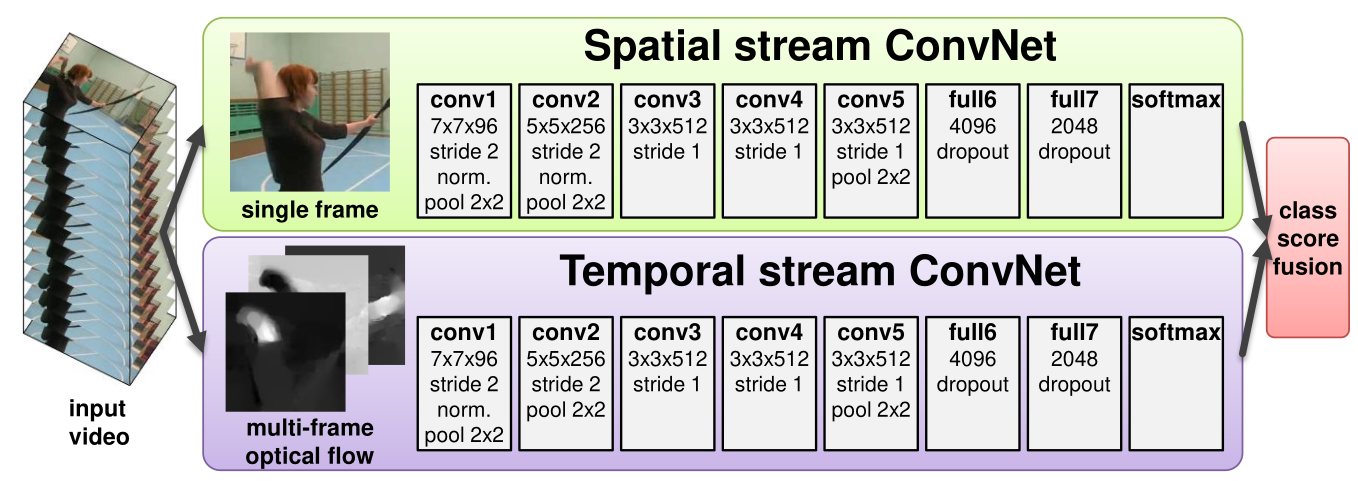
\includegraphics[width=0.99\textwidth]{two-stream-architecture.png}
    \caption{The Two-Stream architecture used by \cite{simonyan_two-stream_2014}. Notice that the spatial and temporal networks have nearly identical architecture, with the difference that the second convolutional layer in the temporal network does not have batch normalization to reduce memory consumption. Image taken from \cite{simonyan_two-stream_2014}. }
    \label{fig:two-stream-architecture}
\end{figure}

In order to improve upon this first approach, \cite{simonyan_two-stream_2014} proposed the \textit{Two-Stream Convolutional neural network}.
Such a network is comprised of two individual networks.
The first network extracts features from a single RGB frame of the video and, by using a softmax layer, classifies the present action.
Simultaneously, the second network processes $L$ consecutive optical flow images and also outputs a classification using a softmax layer.
Both classification outputs are then fed to a multiclass linear Support Vector machine which then outputs the final action prediction.
In \cite{simonyan_two-stream_2014}, the networks have almost the same, shallow architecture, consisting of $5$ convolutional and $2$ fully-connected layers, followed by a softmax layer.
See \fref{fig:two-stream-architecture} for a visualization of the used architecture.

% Spatial
Because the spatial network classifies static images, the authors pretrain it on the ImageNet dataset \cite{deng_imagenet:_2009}.
This step alone improves the accuracy achieved on the UCF101 dataset by $20.5$ percentage points from $52.3$ percent when training from scratch, suggesting that it is highly beneficial to design action recognition architectures in a way that they can be pretrained on large static image datasets.
The authors did not pretrain the temporal network since sufficiently large datasets were not available.

% Flow
The authors evaluated the length of consecutive optical flow frames $L$ of an RGB frame to pass into the flow network.
They noticed that $L=5$ and $L=10$ flow frames lead to similar performance, with $L=10$ being slightly better.
Thus, they decided to set $L=10$.
Additionally, they found that subtracting the mean flow image from every flow frame significantly improved the overall accuracy.
They argue that this is due to the fact that such a subtraction reduces the camera motion, similar to the homography approach by \cite{wang_action_2013} (see \sref{sec:improved-dense-trajectories}).

% Multi Task learning
To train their model, the authors utilized \textit{multi task learning}.
They combined two datasets for training, UCF101 and HMDB51 \cite{kuehne_hmdb:_2011}, 
by changing the architecture so that there are two final softmax layers, one which outputs the prediction for UCF101 and one which outputs the prediction for HMDB51.
The authors found that training in such a way has a regularisation aspect, reducing the risk of overfitting on any of the two datasets.
For computing optical flow, they use the algorithm provided by the OpenCV library \cite{bradski_opencv_2000}.

% Comparison to DenseTrajectories
The authors also evaluated their approach against the Improved Dense Trajectories approach by \cite{wang_action_2013} (see \sref{sec:improved-dense-trajectories}).
On the UCF101 dataset, the Two-Stream network outperformed IDT by $2.1$ percentage points ($85.9$ percent versus $88.0$ percent). 
They argue that this is the case because the Two-Stream network can generalise the HoG, HoF and MBH descriptors used in IDT using its convolutional layers.

\begin{figure}[htb!]
    \centering
    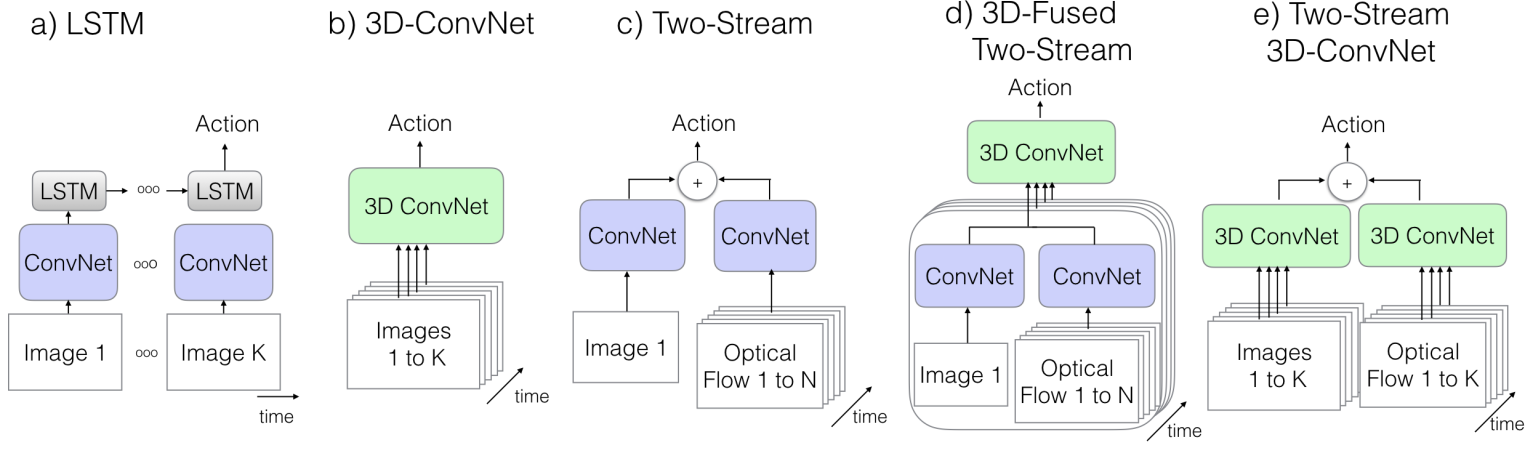
\includegraphics[width=0.99\textwidth]{five-architectures.png}
    \caption{The five architecture types compared in \cite{carreira_quo_2017}. \textbf{e)} is a novel approach proposed by the authors, while \textbf{c)} is the Two-Stream approach proposed by \cite{simonyan_two-stream_2014}. Image taken from \cite{carreira_quo_2017}. }
    \label{fig:five-architectures}
\end{figure}

\subsubsection{Quo Vadis, Action recognition?}
\label{sec:quovadis}
Recently, \cite{carreira_quo_2017} published a video dataset called \textit{Kinetics}, which claims to be big enough to be used for pretraining video processing neural networks, similar to how ImageNet \cite{deng_imagenet:_2009} is used for pretraining static image processing pipelines.
To inspect how much impact such pretraining in the domain of video has the authors reimplemented $5$ popular action recognition architecture types.

First, an architecture where each frame of a video is fed through a 2D convolutional network, whose outputs get aggregated over time using a LSTM layer \cite{hochreiter_long_1997}.
Second, the authors implement a model which uses 3D convolutional layer to process $k$ frames of a video simultaneously.
The idea is that such a model would not need additional temporal components as the 3D layers already capture temporal information.
The architecture is based on \cite{tran_learning_2015}, however, the authors add additional batch normalization to allow for an accurate comparison to other architectures who use batch normalization.
Third, the authors took the Two-Stream architecture by \cite{simonyan_two-stream_2014}.
Fourth, an extension to the Two-Stream architecture by \cite{feichtenhofer_convolutional_2016} is added.
The extension exchanges the fusion stage of the traditional Two-Stream network with 3D convolutional layers.
Also, this approach achieved state-of-the-art results on both UCF101 as well as HMDB51.
Lastly, the authors propose a novel architecture based on both the Two-Stream architecture as well as the 3D convolutional network.
They use two 3D convolutional networks to extract spatial and temporal classifications and then fuse them together, similar to \cite{simonyan_two-stream_2014}.
They utilize a novel approach for pretraining 3D networks by inflating the parameters to the third dimension.
First, they pretrain two 2D networks on ImageNet.
Then, they inflate the convolutional layers filter sizes from $N \times N$ by repeating each filter $N$ times and dividing all filters by $N$.
Thus, they change the dimensionality from $N \times N$ to $N \times N \times N$ for each filter.
They claim that this produces identical output to the 2D network. 
An overview over all $5$ architectures is provided in \fref{fig:five-architectures}.

% Evaluation
For evaluation, the authors pretrained the models on ImageNet and then fine-tuned them on UCF101, HMDB51 as well as Kinetics individually.
In general, they noticed that the Two-Stream approaches outperform the other approaches on all datasets.
The authors argue that this is due to the flow used since the flow network contributes more to the overall accuracy when compared to the spatial network.
Also, they observe that all architectures achieve higher accuracies when pretrained using Kinetics, suggesting that the dataset is suitable for pretraining action recognition models in general.

Moreover, the architecture proposed by the authors achieves state-of-the-art accuracies on both UCF101 ($98$ percent) as well as HMDB51 ($80.7$ percent) when first pretrained on ImageNet, followed by additional pretraining on Kinetics.
The previous state-of-the-art approach by \cite{feichtenhofer_spatiotemporal_2016} achieved $94.5$ and $70.3$ percent, respectively.
The improvement in accuracy over \cite{simonyan_two-stream_2014} is thus $10$ percentage points on UCF101 and $21.3$ percentage points on HMDB51.
Analogously, the performance improvement over \cite{wang_action_2013} is $11.6$ percentage points on UCF101 and $19$ percentage points on HMDB51.
Overall, the authors argue that using Kinetics for pretraining and transfer learning is a feasible approach to achieve similar transfer learning capabilities for video clips as with ImageNet and static images.

\subsection{HAR using pose information}
\label{sec:har_using_pose}
% Towards ...
%TODO: Here, they combine trajectories (positional features) with image features (HOG etc.). This is similar to how Luvizon combines pose and image features!. Can reference back.
\subsubsection{Towards understanding action recognition}
\label{sec:jhuang-towards}
In \cite{jhuang_towards_2013}, the authors evaluate the effect of different parts of a state-of-the-art action recognition pipeline \cite{wang_dense_2013} in order to gain a deeper understanding of the problem (see \sref{sec:dense-trajectories} for a detailed explanation of the algorithm).

In order to evaluate the impact of different parts of an action recognition pipeline they needed a fully annotated dataset.
They took a subset of the HMDB dataset \cite{kuehne_hmdb:_2011}, which they argue is a challenging dataset, and additionally annotated pose and created binary human segmentation maps, which they refer to as Puppet masks (see \sref{sec:exp-jhmdb} for more information on the dataset).

In addition to the annotated poses and Puppet masks, they computed optical flow on consecutive frames for each video clip as well as annotate a rectangular bounding box around the subject.
By substituting ground truth pose, optical flow and bounding boxes into the pipeline of \cite{wang_dense_2013} the authors studied how much these individual features contribute to classification accuracy.

\begin{figure}[htb!]
    \centering
    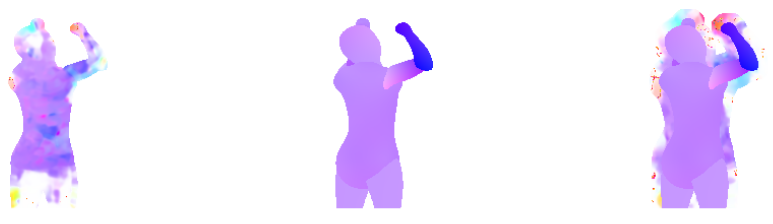
\includegraphics[width=0.6\textwidth]{puppet-flow-mask.png}
    \caption{Three masked optical flow variations used in \cite{jhuang_towards_2013}. \textbf{Left}: The estimated optical flow of \cite{wang_dense_2013} masked using the ground truth Puppet mask annotation. \textbf{Middle}: Optical flow computed only on the masked subject. \textbf{Right}: Combination of both. Notice the sharp edges between the subject and the surrounding flow. Image taken from \cite{jhuang_towards_2013}. }
    \label{fig:puppet-flow-mask}
\end{figure}

To establish a baseline, they extract features using \cite{wang_dense_2013} for each video clip and then train a Support Vector Machine for action classification.
This resulted in an overall accuracy of $56.6$ percent.
Afterwards, they evaluated different ways to substitute the ground truth optical flow into the algorithm.
The highest accuracy gains over the baseline ($11$ percentage points) were achieved by using the ground truth flow computed on the masked subject in combination with using the optical flow from around the Puppet mask borders.
See \fref{fig:puppet-flow-mask} for a visualization.
The authors argue that is most likely due to the fact that the separation between the background flow and subject flow is more distinct, resulting in a sharp motion boundary. 

Next, the authors investigate the impact of masking the subject in the RGB image. 
They use two types of masking. First, they use a bounding box around the subject. Second, they utilize the Puppet mask for masking. 
When applying the masking in such a way that the image is masked before computing the features (as opposed to densely computing features and then masking afterwards) they find that both bounding box masking and puppet flow masking improve significantly upon the baseline with $5.6$ and $8.0$ percentage points respectively.
They argue that the Puppet mask likely leads to a better accuracy because the optical flow algorithm is easier to compute on the subjects boundary.
In addition, they also utilize a state-of-the-art person detector from \cite{bourdev_detecting_2010} to compute the bounding box but find that the computed bounding box is not accurate enough to improve significantly upon the baseline.
This suggests that future progress in person detection algorithm could improve upon current action recognition algorithms.

\begin{figure}[htb!]
    \centering
    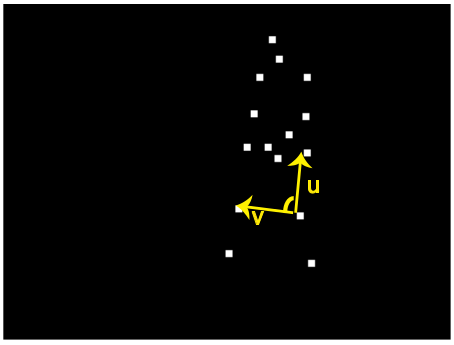
\includegraphics[width=0.3\textwidth]{pose-angle-computation.png}
    \caption{Visualization of computing the inner angle for each joint triplet. The vectors $\bm{u}$ and $\bm{v}$ are calculated from the first joint of each triplet to the other two. Then, the angle between these vectors is computed. Image taken from \cite{jhuang_towards_2013}. }
    \label{fig:joint-angle-computation}
\end{figure}

Afterwards, the impact of using pose as a feature was evaluated.
The authors generate two types of pose related features. 
First, they use the joint positions over time as trajectories. 
Second, they compute additional features related to pose.
This includes calculating the distances and relative angles between all joint pairs. 
In addition, they iterate every triplet of joints and calculate the inner angle spanned by two relative vectors anchored at the third joint.
See \fref{fig:joint-angle-computation} for a visualization of this procedure.
Besides this, they encode temporal information by computing the change in the previously mentioned values for consecutive frames.
They find that the accuracy improves by $19$ percentage points over the baseline, suggesting that pose information is by far the most discriminative feature to use for action recognition \cite{jhuang_towards_2013}. 
Also, adding the image features to the pose features does not significantly improve upon the accuracy. 
The authors thus argue that, once pose features are used, the image feature contribution is negligible.
Additionally, they evaluate the use of estimated poses using the approach presented by \cite{yang_articulated_2011} (see \sref{sec:yangramanan} for a detailed explanation). 
They find that, while the estimated pose is of low quality compared to the ground truth, this approach still outperforms the baseline approach, suggesting that even low quality pose information is highly relevant as a feature for action recognition.

\subsubsection{Pose-CNN}
\label{sec:pcnn}

\begin{figure}[htb!]
    \centering
    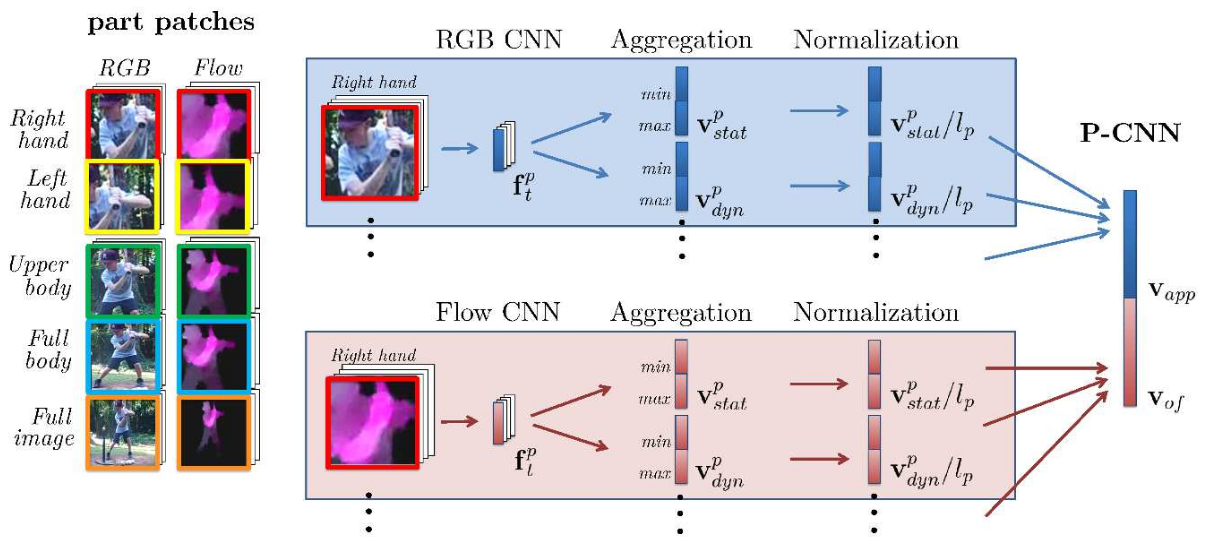
\includegraphics[width=0.99\textwidth]{p-cnn-architecture.png}
    \caption{Visualization of the network architecture used to extract the video descriptor in \cite{cheron_pcnn_2015}. \textbf{In blue}: The part of the Two-Stream network which extracts the visual feature vector $\bm{v_{app}}$. \textbf{In red}: The flow feature extraction network part. Image taken from \cite{cheron_pcnn_2015}. }
    \label{fig:p-cnn-architecture}
\end{figure}

After the findings of \cite{jhuang_towards_2013} discussed previously, \cite{cheron_pcnn_2015} build on their work by proposing a new action descriptor extracted using a Convolutional Neural network.
Specifically, they use a Two-Stream network approach similar to \cite{simonyan_two-stream_2014} (see \sref{sec:two-stream}) where the network is split into two parallel parts.
The first part processes the individual RGB frames, resulting in an appearance feature vector. 
The second part processes flow images and outputs another feature vector. 
These two vectors are then concatenated, which results in the final feature vector for the entire video clip. 
Each part consists of 5 convolutional layers, followed by 3 fully-connected layers. The RGB part is pretrained using the ImageNet dataset \cite{deng_imagenet:_2009} while the flow part is pretrained using the UCF101 dataset \cite{soomro_ucf101:_2012}. 
Once pretrained, the last fully-connected layer of both parts is removed, resulting in a output size of the previous layer of $4096$, which they use as the extracted feature.
See \fref{fig:p-cnn-architecture} for a network visualization.

The authors compute optical flow using \cite{brox_high_2004} for consecutive frames in each video clip beforehand.
They also scale the $x$ and $y$ flow values to the interval $[0, 255]$.
Then, they concatenate these two flow maps and add a third map with the flow magnitude values, resulting in a $3$ channel flow image.
They also preestimate the joint positions using the approach by \cite{yang_articulated_2011}.
Additionally, they use a dynamic programming approach by \cite{cherian_mixing_2014} to refine the estimated pose by incorporating flow information as well as temporal information from previous and following poses.
Afterwards, using the precomputed joint positions, they extract subimages around the right hand, left hand, upper body, full body and full image from the RGB frames as well as from the flow images.

After passing all subimages through the network, the resulting feature vectors $f_t^p$ for time step $t$ and body part $p$ are aggregated by first computing minimum and maximum values $m_i, M_i$ for each descriptor dimension $i$.
Then, the minimum values for each dimension are concatenated, followed by another concatenation of the maximum values.
The authors refer to this vector as the static video descriptor since it is computed per frame without taking future or past frames into account.
They compute another descriptor, called the dynamic video descriptor, where the original feature descriptors $f_t^p$ get subtracted by $f_{(t-4)}^p$, thus encoding temporal information.
The aggregation of minimum and maximum values following that is identical to the aggregation for the static video descriptor.
Finally, both descriptors are normalized and again concatenated, yielding the final video descriptor.
The resulting feature vector is then used as input for a linear Support Vector Machine, used for action classification.
See \fref{fig:p-cnn-architecture} for a visualization.

The authors compare their results to the descriptor presented in \sref{sec:jhuang-towards} (from now on referred to as \textit{HLPF} for High Level Pose Features) as well as to the Improved Dense Trajectories (\textit{IDT}) descriptor presented in \sref{sec:improved-dense-trajectories}, which was the state-of-the-art approach at that time.

When training on the JHMDB dataset, the authors find that their approach does not outperform \textit{HLPF} when using ground truth pose annotations ($74.6$ and $77.8$ percent accuracy respectively).
However, when using estimated pose, their approach significantly outperforms \textit{HLPF} by almost $35$ percentage points ($61.1$ as opposed to $25.3$).
While the authors give no explanation for why this might be the case, one possibility would be that the conclusion of \cite{jhuang_towards_2013} that visual features and flow do not significantly improve upon accuracy when also utilizing pose might not hold in all situations.
For example, consider two actions like \textit{military salute} and \textit{talking on the phone}, which have similar poses.
When also considering image features, the distinction between an empty hand (\textit{military salute}) and a hand containing an object (\textit{talking on the phone}) can aid in the decision process.
Also, since the authors use a different approach for estimating pose as opposed to \cite{jhuang_towards_2013} and they do not evaluate the accuracy of the pose estimator individually it might be the case that the pose information itself is not of sufficient quality for the pose features computed by \textit{HLPF} to be discriminative enough.

Interestingly, the authors find that, while their approach does not outperform \textit{IDT}, a combination of their descriptor with \textit{IDT} significantly outperforms \textit{IDT} on its own.
The authors argue that, because \textit{IDT} uses a larger time window for feature aggregation, actions like \textit{kick ball} achieve higher accuracy while on actions like \textit{shoot gun} and \textit{waving} the image features extracted by their method provide more information and thus higher accuracy.
A combination thus improves the accuracy in both scenarios simultaneously.
%- TODO: Explain Fisher Vector (Improving the Fisher kernel for large-scale image classification)

\subsubsection{PoTion}
\label{sec:potion}

\begin{figure}[htb!]
    \centering
    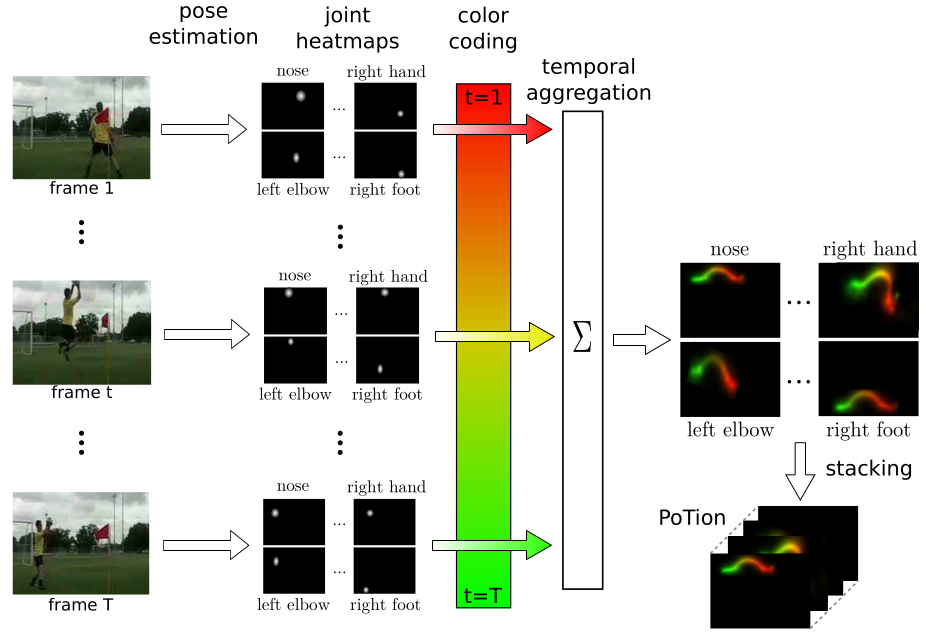
\includegraphics[width=0.9\textwidth]{potion-overview.png}
    \caption{The approach presented in \cite{choutas_potion:_2018} first estimates the joint positions for each frame of a video. Then, depending on the frame, the position is colored according to a gradient from, for example, red to green. By aggregating all frames in to a single image the path the joint moved in the frame becomes visible. Image taken from \cite{choutas_potion:_2018}. }
    \label{fig:potion-overview}
\end{figure}

% Intro + general approach
Building on the work of \cite{simonyan_two-stream_2014} (see \sref{sec:two-stream}), \cite{choutas_potion:_2018} propose a complementary pose-based feature called \textit{Pose motion (PoTion)}.
The idea is to track joint positions over time and displaying them in a single frame using a color gradient.
The authors argue that such a compact representation can be used in combination to recent Two-Stream approaches to achieve state-of-the-art performance.
See \fref{fig:potion-overview} for a visualization of this approach.

First, the authors compute joint positions for each frame of a clip using a pose estimator proposed in \cite{cao_realtime_2017}.
Then, the authors define $C$ colors to encode the movement for each joint.
Using a gradient between these colors, the authors color each joint position based on the frame position in the video.
For example, consider $C=2$ and let these two colors be red and green.
Then, the joints in the first frame would be colored red.
Analogously, the joints in the last frame would be colored green.
In between, the authors define a function for interpolating between the different colors.
Notice that the color is solely dependent on the frame position $t$.
See \fref{fig:potion-color} for a visualization of these functions. 
In their evaluation, the authors find that, initially, the accuracy on the datasets increases with the number of colors used.
They find that this is the case until $C=6$, where the accuracy stops increasing.
Thus, the authors choose $C=4$ in order to get both a high accuracy and remain a compact representation.

\begin{figure}[htb!]
    \centering
    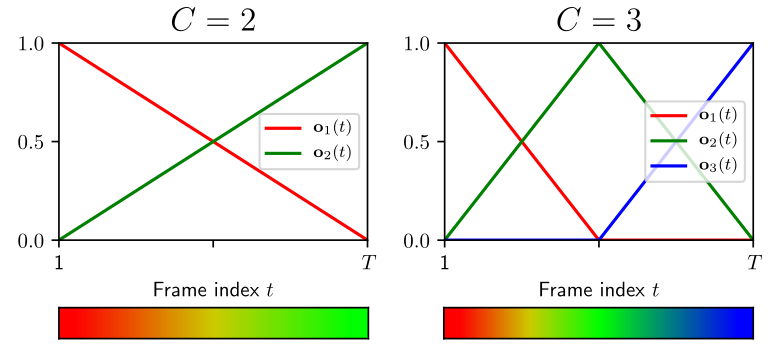
\includegraphics[width=0.7\textwidth]{potion-color.png}
    \caption{Example of the color interpolation for two and three different colors. On the bottom, the resulting color for each frame $t$ is shown. Image taken from \cite{choutas_potion:_2018}. }
    \label{fig:potion-color}
\end{figure}

Afterwards, the authors aggregate the colorized frames for each joint into a single RGB image.
They evaluate different aggregation techniques.
First, they compute the normalized sum $U_j$ for each joint $j$ by summing all colorized frames and dividing by the maximum pixel value over all pixels.
The authors notice that, if a joint stays at any position for a period of time, that the intensity increases strongly at this particular position.
Thus, they also compute an intensity image $I_j = \sum_c U_j(c)$ by summing all color channels for all pixels in $U_j$.
Then, they compute an additional representation $N_j = \frac{U_J}{\epsilon + I_j}$, which does not contain intensity information.
In their evaluation, the authors find they achieve the highest accuracy by using all three representations.

For evaluation, the authors also propose a shallow CNN for classification using only the precomputed representations discussed earlier.
The network is made up of $6$ convolutional layers, followed by a single full-connected layer.
However, the authors find that this shallow classification network alone does not achieve high accuracies compared to the previous work.
On the JHMDB dataset, the authors achieve $57.0$ percent accuracy (as compared to $61.1$ percent achieved by \cite{cheron_pcnn_2015} (see \sref{sec:pcnn})) and on HMDB, the authors achieve $43.7$ percent accuracy (as compared to $59.4$ and $61.7$ percent by \cite{simonyan_two-stream_2014} (see \sref{sec:two-stream}) and \cite{wang_action_2013} \sref{sec:improved-dense-trajectories} respectively).

The authors also evaluate the effect of adding their representation to other previous approaches and find that adding it to the previous state-of-the-art approach by \cite{carreira_quo_2017} (see \sref{sec:quovadis}) they were able to improve the accuracy slightly by $0.5$ ($87.9$ percent as opposed to $87.4$ percent) percentage points using estimated poses on the JHMDB dataset.
When using ground truth annotation for the joint positions, the authors observe an improvement of $3$ percentage points to $90.4$ percent upon \cite{carreira_quo_2017}, indicating that their representation is complementary to the Two-Stream approach and that it is worthwhile to improve upon the pose estimation component.

\subsubsection{Three-Stream Network}
\label{sec:three-stream}

Inspired by the success of the Two-Stream architecture (see \sref{sec:two-stream}), \cite{khalid_multi-modal_2018} expanded the idea to a Three-Stream approach, using pose information as the third stream.

% Pose Tensor
First, they estimate the poses for each frame using the same pose estimator by \cite{cao_realtime_2017} that \cite{choutas_potion:_2018} use.
%% Missing Joints (two interpolation techniques)
The authors argue, however, that missing joints need to be interpolated because this leads to higher accuracy on the benchmark datasets.
However, they do not provide evidence in form of a direct comparison of accuracy with and without interpolation.
They propose two different interpolation strategies, referred to as \textit{temporal interpolation} and \textit{spatial interpolation}.
\textit{Temporal interpolation} is used whenever a joint is not visible for a small number of frames.
Let $f_l$ be the frame where the joint was last visible.
This frame is then followed by $n$ frames, where it is not visible, followed by $f_k$, where it becomes visible again.
Then, the authors linearly interpolate the position of the missing joint for each frame $f_{l+1}, \dots, f_{l+n}$ using the positions in $f_l$ and $f_k$.
They do, however, not specify what constitutes as a \textit{small number of frames}, i.e., how small $n$ has to be in order for this approach to lead to good results.
\textit{Spatial interpolation} is used for long-term occlusion, i.e., for large $n$.
The authors argue that this is necessary since \textit{temporal interpolation} leads to worse results the bigger $n$ gets.
Again, they do not specify for which value of $n$ \textit{spatial interpolation} becomes necessary.
For \textit{spatial interpolation}, they divide the joints into $5$ groups, which can be seen in \fref{fig:khalid-joint-groups}.
The groups are iterated, starting with the group the missing joint is in.
If the other joints in a group are present, they \textit{vote} on the position of the missing joints based on a statistical model of relative joint positions computed on training data beforehand.
The average vote is then assumed to be the missing joints position.
The authors argue that this leads to good results since the position of joints is highly correlated for certain joints.
As an example, they mention the correlation of head and neck positions.
This approach and reasoning is similar to \cite{yang_articulated_2011} (see \sref{sec:yangramanan}), where the relative orientation between joints was used as a feature for action recognition.

\begin{figure}[htb!]
    \centering
    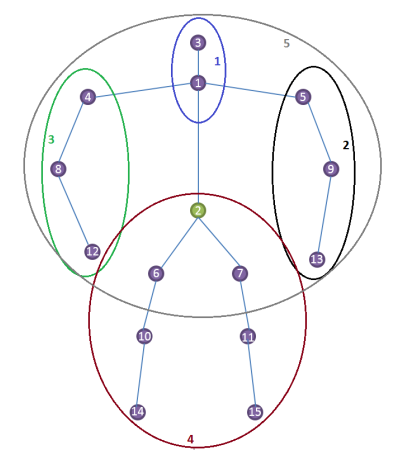
\includegraphics[width=0.3\textwidth]{khalid-joint-groups.png}
    \caption{The authors divide the joints into $5$ groups in order to estimate relative positions of joints to each other. Image taken from \cite{khalid_multi-modal_2018}. }
    \label{fig:khalid-joint-groups}
\end{figure}

Once the joint positions are estimated for each frame, the authors order them in a way so that the neighbourhood relationship between joints is kept.
They argue that this leads to higher accuracy since the relationship of the joints is a useful feature, but they do not compare it to other approaches for joint ordering.
The ordering process is visualized in \fref{fig:khalid-pose-tensor}.
By traversing the tree in such a way, some nodes are visited multiple times and thus present multiple times in the pose tensor.
That way, the authors argue, neighbourhood relationships are expressed more directly in comparison to simply starting at joint $1$ and concatenating the $x$ and $y$ positions.
The pose tensor then contains the $x$ and $y$ information for each frame in a row.
The authors process the video clips in chunks, so that the pose tensor always has identical dimensions.
Also, in the second and third tensor dimension they compute the first and second order derivatives of the joint position coordinates.
Finally, the joint positions $P_i$ are normalized with regards to the middle point between \textit{neck} and \textit{belly} joint $P_{middle}$ and with regards to the torso length $d$ using the following two formulas:

\begin{equation}
    P^{norm}_i = \frac{P_i}{d}, \\
    P^{rel}_i = P^{norm}_i - P_{middle}.
\end{equation}

\begin{figure}[htb!]
    \centering
    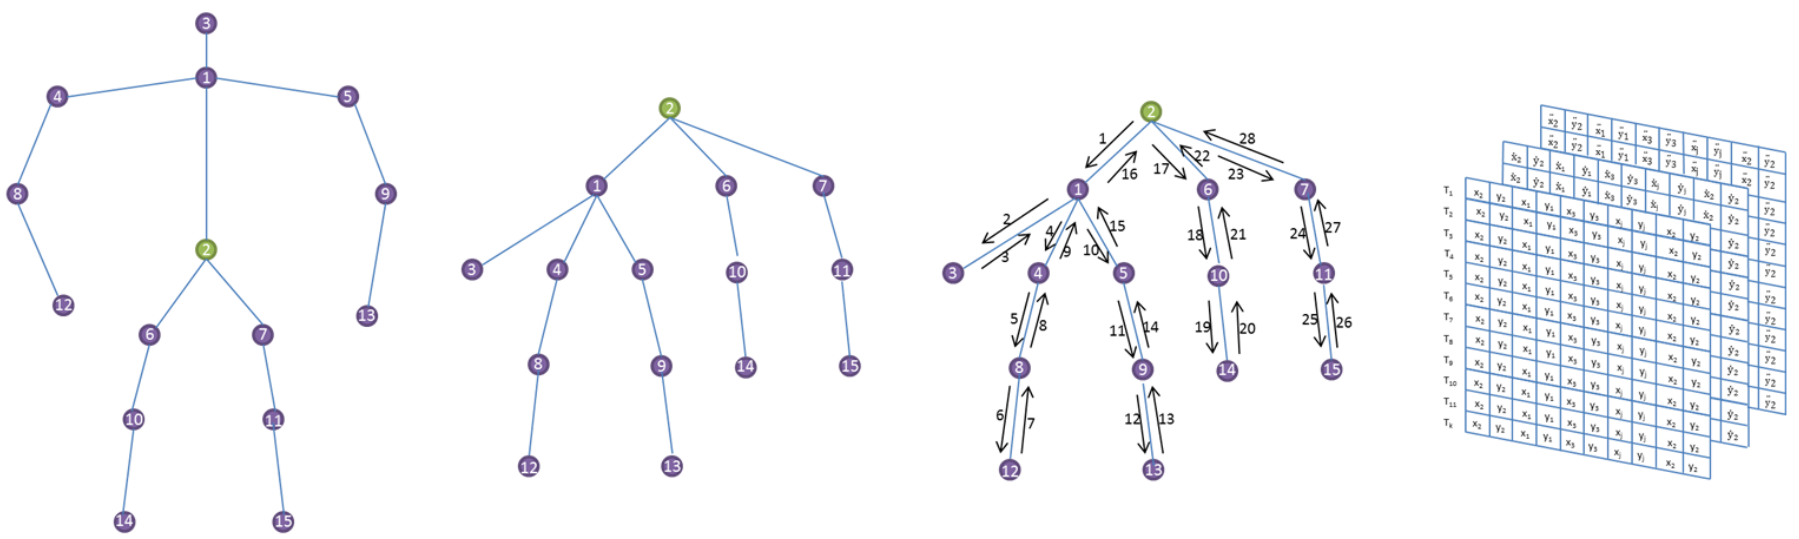
\includegraphics[width=0.99\textwidth]{khalid-pose-tensor.png}
    \caption{Visualization of the ordering process. \textbf{From left to right}: \textbf{a)} The original pose skeleton. The belly joint is highlighted and used as the root node. \textbf{b)} A tree is computed based on the previously chosen root node. \textbf{c)} Traversion algorithm example. \textbf{d)} The final pose vector. Each row contains $x$ and $y$ coordinates of the persons joint locations of one frame. Image taken from \cite{khalid_multi-modal_2018}. }
    \label{fig:khalid-pose-tensor}
\end{figure}

% Pose ConvNet
The authors propose a shallow CNN for classification, similar to the one proposed by \cite{choutas_potion:_2018} (see \sref{sec:potion}).
The network is made up of two convolutional layers, followed by a max pooling layer and a fully-connected layer.
Finally, a layer with the softmax activation function is used for classification.
The other layers all utilize the ReLU activation function.
Since the network is so small, the authors do not pretrain it.
For the Two-Stream architecture, they use \cite{wang_temporal_2016}, which is a Two-Stream network achieving high accuracy on the UCF101 and HMDB datasets.
They fuse their pose network into the existing Two-Stream approach by equally weighting all three components. 

% Evaluation
First, the authors evaluate each component of the Three-Stream architecture independently and find that the pose component (using estimated pose) and spatial component perform worse than the components using optical flow and ground truth pose components, suggesting the importance of motion information for action recognition.
When combining the different components, the Three-Stream network performs the best with $78.81$ percent accuracy on the JHMDB dataset using estimated pose.
When substituting ground truth pose, the accuracy further increases to $83.05$ percent.

When comparing the Three-Stream network to previously discussed methods, it performs slightly worse ($0.7$ percentage points) on the JHMDB dataset, using estimated pose, when compared to \cite{cheron_pcnn_2015} (see \sref{sec:pcnn}).
Even when utilizing ground truth pose information, the authors are not able to outperform \cite{choutas_potion:_2018}, who achieved $87.9$ percent accuracy on JHMDB using estimated pose.
Notice that the pose estimator was identical in both cases, suggesting that either the architecture proposed by \cite{khalid_multi-modal_2018} is not deep enough or that estimating missing joint positions by linear interpolation and statistical modeling leads to worse results.
